% Options for packages loaded elsewhere
\PassOptionsToPackage{unicode}{hyperref}
\PassOptionsToPackage{hyphens}{url}
\documentclass[
  ignorenonframetext,
  aspectratio=169,
]{beamer}
\newif\ifbibliography
\usepackage{pgfpages}
\setbeamertemplate{caption}[numbered]
\setbeamertemplate{caption label separator}{: }
\setbeamercolor{caption name}{fg=normal text.fg}
\beamertemplatenavigationsymbolsempty
% remove section numbering
\setbeamertemplate{part page}{
  \centering
  \begin{beamercolorbox}[sep=16pt,center]{part title}
    \usebeamerfont{part title}\insertpart\par
  \end{beamercolorbox}
}
\setbeamertemplate{section page}{
  \centering
  \begin{beamercolorbox}[sep=12pt,center]{section title}
    \usebeamerfont{section title}\insertsection\par
  \end{beamercolorbox}
}
\setbeamertemplate{subsection page}{
  \centering
  \begin{beamercolorbox}[sep=8pt,center]{subsection title}
    \usebeamerfont{subsection title}\insertsubsection\par
  \end{beamercolorbox}
}
% Prevent slide breaks in the middle of a paragraph
\widowpenalties 1 10000
\raggedbottom
\AtBeginPart{
  \frame{\partpage}
}
\AtBeginSection{
  \ifbibliography
  \else
    \frame{\sectionpage}
  \fi
}
\AtBeginSubsection{
  \frame{\subsectionpage}
}
\usepackage{iftex}
\ifPDFTeX
  \usepackage[T1]{fontenc}
  \usepackage[utf8]{inputenc}
  \usepackage{textcomp} % provide euro and other symbols
\else % if luatex or xetex
  \usepackage{unicode-math} % this also loads fontspec
  \defaultfontfeatures{Scale=MatchLowercase}
  \defaultfontfeatures[\rmfamily]{Ligatures=TeX,Scale=1}
\fi
\usepackage{lmodern}
\ifPDFTeX\else
  % xetex/luatex font selection
\fi
% Use upquote if available, for straight quotes in verbatim environments
\IfFileExists{upquote.sty}{\usepackage{upquote}}{}
\IfFileExists{microtype.sty}{% use microtype if available
  \usepackage[]{microtype}
  \UseMicrotypeSet[protrusion]{basicmath} % disable protrusion for tt fonts
}{}
\makeatletter
\@ifundefined{KOMAClassName}{% if non-KOMA class
  \IfFileExists{parskip.sty}{%
    \usepackage{parskip}
  }{% else
    \setlength{\parindent}{0pt}
    \setlength{\parskip}{6pt plus 2pt minus 1pt}}
}{% if KOMA class
  \KOMAoptions{parskip=half}}
\makeatother
\usepackage{longtable,booktabs,array}
\usepackage{caption}
\captionsetup[table]{skip=6pt}
\newcounter{none} % for unnumbered tables
\usepackage{calc} % for calculating minipage widths
\usepackage{caption}
% Make caption package work with longtable
\makeatletter
\def\fnum@table{\tablename~\thetable}
\makeatother
\usepackage{graphicx}
\makeatletter
\newsavebox\pandoc@box
\newcommand*\pandocbounded[1]{% scales image to fit in text height/width
  \sbox\pandoc@box{#1}%
  \Gscale@div\@tempa{\textheight}{\dimexpr\ht\pandoc@box+\dp\pandoc@box\relax}%
  \Gscale@div\@tempb{\linewidth}{\wd\pandoc@box}%
  \ifdim\@tempb\p@<\@tempa\p@\let\@tempa\@tempb\fi% select the smaller of both
  \ifdim\@tempa\p@<\p@\scalebox{\@tempa}{\usebox\pandoc@box}%
  \else\usebox{\pandoc@box}%
  \fi%
}
% Set default figure placement to htbp
\def\fps@figure{htbp}
\makeatother
\setlength{\emergencystretch}{3em} % prevent overfull lines
\providecommand{\tightlist}{%
  \setlength{\itemsep}{0pt}\setlength{\parskip}{0pt}}
% Auto-generated by infrastructure/rendering/_pdf_latex_helpers.py::extract_math_font_preamble.
% Minimal header passed to Pandoc via -H so Beamer slides pick up the same math font
% as the combined-PDF path. Adjust the manuscript's preamble.md to change the font globally.
\usepackage{unicode-math}
\setmathfont{latinmodern-math.otf}

% Manuscript macro/package fallbacks (newcommand -> providecommand).
% Core mathematics
\usepackage{amsmath}
\usepackage{amssymb}
% Document layout
% Tables
\usepackage{booktabs}
% Caption styling (booktabs already loaded above). Small caption font with a
% bold label ("Figure 1", "Table 2") gives the math/figure-heavy layout a
% consistent, journal-like caption rhythm without fighting pandoc-crossref —
% pandoc emits standard \caption{}, and caption/captionsetup only restyle it.
% ── Theorem environments ─────────────────────────────────────────────────
% amsthm is loaded above. The FedGVI<->Friston bridge is stated as a small
% number of theorems/definitions/lemmas/propositions/corollaries; sharing one
% counter (definition/lemma/proposition/corollary all step the `theorem`
% counter) gives a single monotone numbering 1, 2, 3, ... across all kinds, so
% authors can reference them as Theorem 1, Definition 2, Corollary 3 without a
% per-kind counter drifting out of order. Plain style for theorem-like results,
% definition style (upright body) for definitions.
% (algorithm2e intentionally not loaded: this manuscript states results as
% numbered amsthm Theorems/Definitions, not algorithm2e pseudocode.)
% Code listings
\usepackage{listings}
% Typography and formatting
% (siunitx intentionally not loaded: no \SI/\num units appear in this manuscript.)
% Cross-references and citations
% (cleveref and titlesec intentionally not loaded: unavailable in this TeX tree
% and not required. Cross-references resolve through pandoc-crossref's own
% \ref-style names — no \cref appears — and section heading styling falls back
% to the pandoc/LaTeX defaults.)
% ── TeX Live Basic-compatible mono font for code listings ────────────
% Latin Modern Mono is bundled with TeX Live Basic and keeps the manuscript
% renderable on minimal TeX installations. Mathematical Unicode coverage is
% provided separately by Latin Modern Math below, so the code font does not
% need a private JuliaMono installation.
%
% Use the TeX font filename rather than the system-family name: the minimal
% TeX Live fontconfig database may not register the OpenType family even though
% kpsewhich can resolve the bundled files.
% Math font for unicode-math: Latin Modern Math (TeX Live) has full BMP
% coverage including U+2223 (\mid), U+226A/226B (\ll/\gg), and the Greek/
% blackboard letters used in equations. Without an explicit \setmathfont,
% unicode-math falls back to lmroman text font which lacks several glyphs
% and emits "Missing character" warnings on every \mid in math mode.

% Slide layout defaults for warning-clean scientific decks.
\usepackage{etoolbox}
\IfFileExists{xurl.sty}{\usepackage{xurl}}{}
\IfFileExists{seqsplit.sty}{\usepackage{seqsplit}}{\newcommand{\seqsplit}[1]{#1}}
\protected\def\breakseq#1{\seqsplit{#1}}
\protected\def\breaktt#1{\begingroup\ttfamily\seqsplit{#1}\endgroup}
\setlength{\emergencystretch}{6em}
\tolerance=5000
\hbadness=10000
\hfuzz=1pt
\setlength{\tabcolsep}{2pt}
\AtBeginEnvironment{longtable}{\tiny\renewcommand{\arraystretch}{0.86}\setlength{\tabcolsep}{1pt}}
\AtBeginEnvironment{tabular}{\tiny\renewcommand{\arraystretch}{0.86}\setlength{\tabcolsep}{1pt}}
\AtBeginEnvironment{equation}{\tiny}
\AtBeginEnvironment{equation*}{\tiny}
\AtBeginEnvironment{align}{\tiny}
\AtBeginEnvironment{align*}{\tiny}
\AtBeginEnvironment{itemize}{\footnotesize}
\AtBeginEnvironment{enumerate}{\footnotesize}
\AtBeginEnvironment{description}{\footnotesize}
\setbeamerfont{caption}{size=\tiny}
\setbeamerfont{caption name}{size=\tiny}
\setbeamerfont{normal text}{size=\small}
\setbeamerfont{frametitle}{size=\small}
\setbeamerfont{section title}{size=\footnotesize}
\setbeamerfont{subsection title}{size=\footnotesize}
\setbeamertemplate{section page}{%
  \centering
  \begin{beamercolorbox}[sep=12pt,center,wd=\paperwidth]{section title}
    \parbox{0.86\paperwidth}{\centering\usebeamerfont{section title}\insertsection\par}
  \end{beamercolorbox}
}
\setbeamertemplate{subsection page}{%
  \centering
  \begin{beamercolorbox}[sep=8pt,center,wd=\paperwidth]{subsection title}
    \parbox{0.86\paperwidth}{\centering\usebeamerfont{subsection title}\insertsubsection\par}
  \end{beamercolorbox}
}
\setlength{\abovecaptionskip}{2pt}
\setlength{\belowcaptionskip}{0pt}

% Natbib and cross-reference fallbacks — slides don't load natbib
% or cleveref, but combined-PDF manuscript prose may emit these
% commands. The fallback renders citations as a bracketed key list
% and cross-references as detokenized labels so slides don't fail on
% undefined control sequences or raw underscores. \providecommand is
% a no-op if packages load later.
\providecommand{\citep}[1]{[#1]}
\providecommand{\citet}[1]{#1}
\providecommand{\citealp}[1]{#1}
\providecommand{\citeauthor}[1]{#1}
\providecommand{\citeyear}[1]{#1}
\providecommand{\cref}[1]{\texttt{\detokenize{#1}}}
\providecommand{\Cref}[1]{\texttt{\detokenize{#1}}}
\providecommand{\crefrange}[2]{\texttt{\detokenize{#1}}--\texttt{\detokenize{#2}}}
\providecommand{\Crefrange}[2]{\texttt{\detokenize{#1}}--\texttt{\detokenize{#2}}}
\providecommand{\paragraph}[1]{\textbf{#1}\ }

% Opt-in accessible presentation profile.
\setbeamerfont{normal text}{size*={20pt}{24pt}}
\setbeamerfont{frametitle}{size*={28pt}{32pt}}
\setbeamerfont{section title}{size*={28pt}{32pt}}
\setbeamerfont{subsection title}{size*={28pt}{32pt}}
\setbeamerfont{caption}{size*={16pt}{19pt}}
\setbeamerfont{caption name}{size*={16pt}{19pt}}
\setbeamerfont{itemize/enumerate body}{size*={20pt}{24pt}}
\setbeamerfont{itemize/enumerate subbody}{size*={20pt}{24pt}}
\setbeamerfont{itemize/enumerate subsubbody}{size*={20pt}{24pt}}
\setbeamerfont{itemize item}{size*={20pt}{24pt}}
\setbeamerfont{itemize subitem}{size*={20pt}{24pt}}
\setbeamerfont{itemize subsubitem}{size*={20pt}{24pt}}
\setbeamerfont{description body}{size*={20pt}{24pt}}
\setbeamerfont{description item}{size*={20pt}{24pt}}
\setbeamerfont{quote}{size*={20pt}{24pt}}
\setbeamerfont{quotation}{size*={20pt}{24pt}}
\AtBeginEnvironment{longtable}{\fontsize{20pt}{24pt}\selectfont}
\AtBeginEnvironment{tabular}{\fontsize{20pt}{24pt}\selectfont}
\AtBeginEnvironment{equation}{\fontsize{20pt}{24pt}\selectfont}
\AtBeginEnvironment{equation*}{\fontsize{20pt}{24pt}\selectfont}
\AtBeginEnvironment{align}{\fontsize{20pt}{24pt}\selectfont}
\AtBeginEnvironment{align*}{\fontsize{20pt}{24pt}\selectfont}
\AtBeginEnvironment{itemize}{\fontsize{20pt}{24pt}\selectfont}
\AtBeginEnvironment{enumerate}{\fontsize{20pt}{24pt}\selectfont}
\AtBeginEnvironment{description}{\fontsize{20pt}{24pt}\selectfont}
\AtBeginDocument{\usebeamerfont{normal text}}
\newlength{\AFSlideTableWidth}
% The fixed footer reservation is calibrated with the semantic seven-line regular-body budget.
\setbeamertemplate{footline}{%
  \leavevmode\vbox{%
    \hbox{%
      \begin{beamercolorbox}[wd=\paperwidth,ht=16pt,dp=3pt,center]{author in head/foot}%
        \fontsize{16pt}{19pt}\selectfont Untagged PDF derivative \textbar\ \href{../web/index.html}{HTML reader}%
      \end{beamercolorbox}%
    }%
    \vskip6pt%
  }%
}
% Accessible footer reserved height: 25pt.

\newtheorem{proposition}{Proposition}
\newtheorem{hypothesis}{Hypothesis}
\newtheorem{remark}[theorem]{Remark}
\newtheorem{axiom}{Axiom}
\newtheorem{property}{Property}
\usepackage{bookmark}
\IfFileExists{xurl.sty}{\usepackage{xurl}}{} % add URL line breaks if available
\urlstyle{same}
% fallback for those not using the hyperref driver hyperxmp:
\makeatletter
\@ifundefined{xmpquote}{\newcommand{\xmpquote}[1]{#1}}{}
\makeatother
\hypersetup{
  hidelinks,
  pdfcreator={LaTeX via pandoc}}

\author{\texorpdfstring{}{}}
\date{}

\begin{document}

\begin{frame}{Generative model: categorical states, observations,
actions, and hierarchy}
\protect\phantomsection\label{sec:methods-generative-model}
The 9 studies --- including the contaminated-sentinel robustness sweep
(Study 4) --- run on one shared sentinel world (Studies 5--7 use its
moving and hierarchical variants):
\end{frame}

\begin{frame}{Generative model (part 2)}
a discrete sentinel partially-observable Markov decision process (POMDP)
using the categorical world structure illustrated by Friston et al.
(2024), Figures 1 and 4.
\end{frame}

\begin{frame}[fragile]{Generative model (part 3)}
We adopt the discrete-state active-inference formulation that the
community has standardized around --- the categorical \(A/B/C/D_0\)
generative model of da Costa et al. (2020), the same object the
\texttt{pymdp} (Heins et al. 2022) and RxInfer (Bagaev et al. 2023)
toolboxes operate on.
\end{frame}

\begin{frame}[fragile]{Generative model (part 4)}
We reimplement it in pure NumPy in \texttt{pomdp.py} so the colony, its
sensors, and its dynamics are exactly the ones the analysis executes.

A colony of sentinels watches a single hidden creature whose location is
the shared latent factor they federate beliefs about.
\end{frame}

\begin{frame}{Generative model (part 5)}
The structural map in fig.~4 follows the
same generative-model vocabulary while making the implementation
boundary visible: Panel A shows what one agent actually sees --- one
noisy categorical report over the 9 possible locations ---
\end{frame}

\begin{frame}{Generative model (part 6)}
while Panel B identifies the \(A/B/C/D_0\) factors that turn that report
into a local posterior.
\end{frame}

\begin{frame}{Generative model (part 7)}
Temporal depth then describes state, observation, posterior, and control
order; hierarchical depth describes conditioned priors. It is a formal
schematic, not an assertion that every displayed dependency is
simultaneously estimated in every study.
\end{frame}

\begin{frame}{Generative model (part 8)}
\begin{figure}
\centering
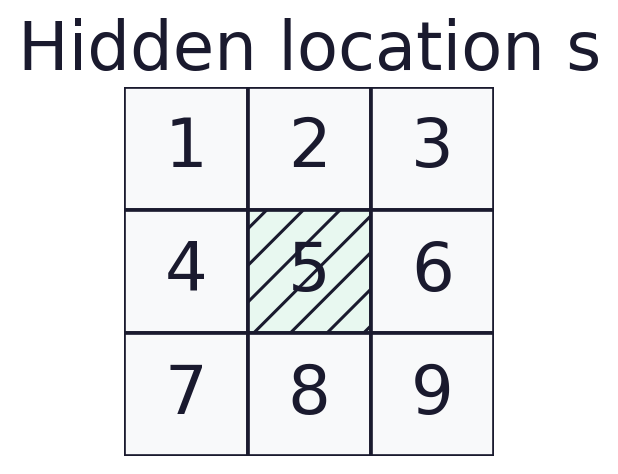
\includegraphics[keepaspectratio,width=0.98\linewidth,height=0.8\textheight,alt={Hidden location s: nine-cell topology; cell 5 is hatched. Schematic only, no measured probability scale.}]{../figures/generative_model_schema.slide-hidden-location.png}
\refstepcounter{figure}\label{fig:generative-model-schema-slide-panel-1}
\end{figure}
\end{frame}

\begin{frame}{Generative model (part 9)}
\begin{figure}
\centering
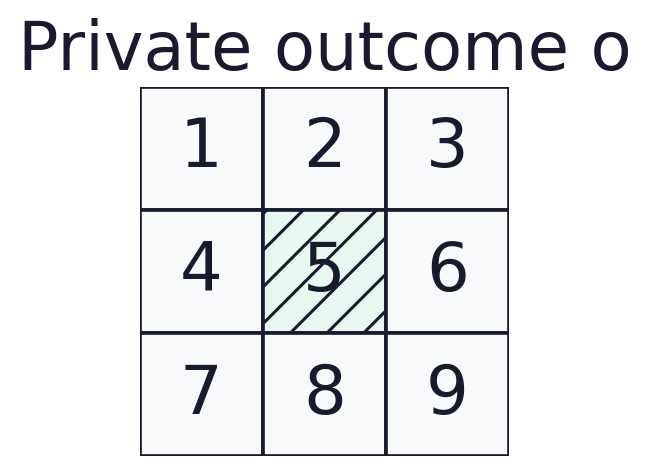
\includegraphics[keepaspectratio,width=0.98\linewidth,height=0.8\textheight,alt={Private outcome o: nine-cell topology; cell 5 is hatched. Schematic only, no measured probability scale.}]{../figures/generative_model_schema.slide-outcome.png}
\refstepcounter{figure}\label{fig:generative-model-schema-slide-panel-2}
\end{figure}
\end{frame}

\begin{frame}{Generative model (part 10)}
\begin{figure}
\centering
\includegraphics[keepaspectratio,width=0.98\linewidth,height=0.8\textheight,alt={Hidden location s \texorpdfstring{\ensuremath{\to}}{->} Private outcome o: A{[}o,s{]} = P(o\textbar s); data\_dependency.}]{../figures/generative_model_schema.slide-sensor.png}
\refstepcounter{figure}\label{fig:generative-model-schema-slide-panel-3}
\end{figure}
\end{frame}

\begin{frame}{Generative model (part 11)}
\begin{figure}
\centering
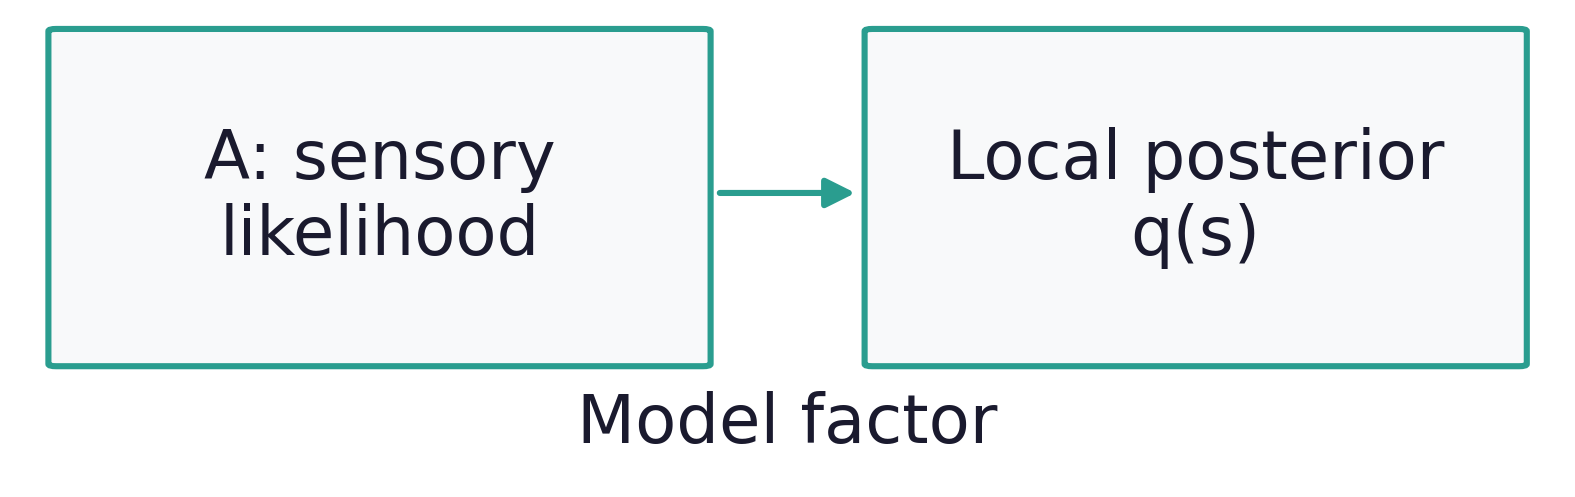
\includegraphics[keepaspectratio,width=0.98\linewidth,height=0.8\textheight,alt={A: sensory likelihood → Local posterior q(s): Model factor; data\_dependency.}]{../figures/generative_model_schema.slide-likelihood.png}
\refstepcounter{figure}\label{fig:generative-model-schema-slide-panel-4}
\end{figure}
\end{frame}

\begin{frame}{Generative model (part 12)}
\begin{figure}
\centering
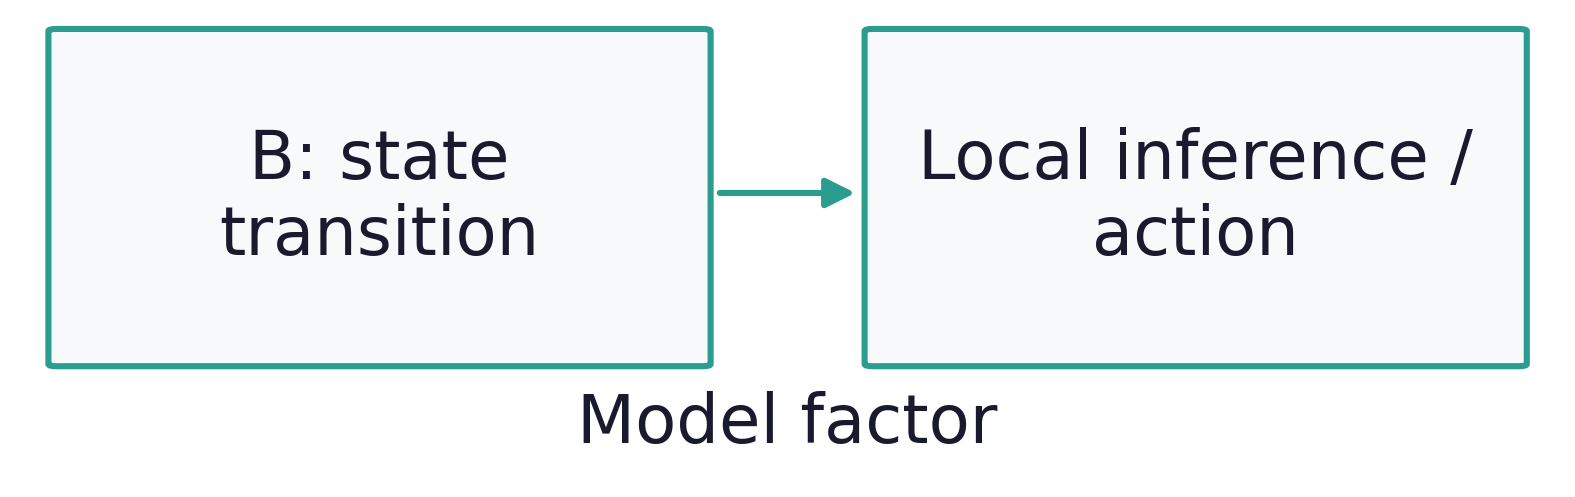
\includegraphics[keepaspectratio,width=0.98\linewidth,height=0.8\textheight,alt={B: state transition → Local inference / action: Model factor; data\_dependency.}]{../figures/generative_model_schema.slide-dynamics.png}
\refstepcounter{figure}\label{fig:generative-model-schema-slide-panel-5}
\end{figure}
\end{frame}

\begin{frame}{Generative model (part 13)}
\begin{figure}
\centering
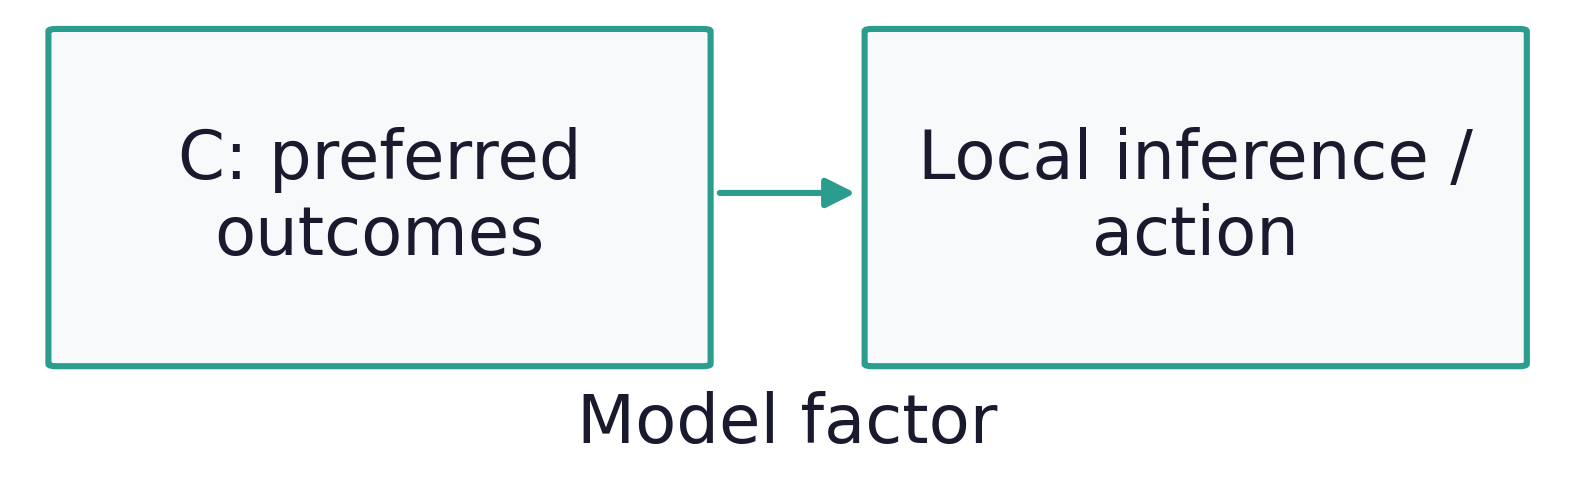
\includegraphics[keepaspectratio,width=0.98\linewidth,height=0.8\textheight,alt={C: preferred outcomes → Local inference / action: Model factor; data\_dependency.}]{../figures/generative_model_schema.slide-preferences.png}
\refstepcounter{figure}\label{fig:generative-model-schema-slide-panel-6}
\end{figure}
\end{frame}

\begin{frame}{Generative model (part 14)}
\begin{figure}
\centering
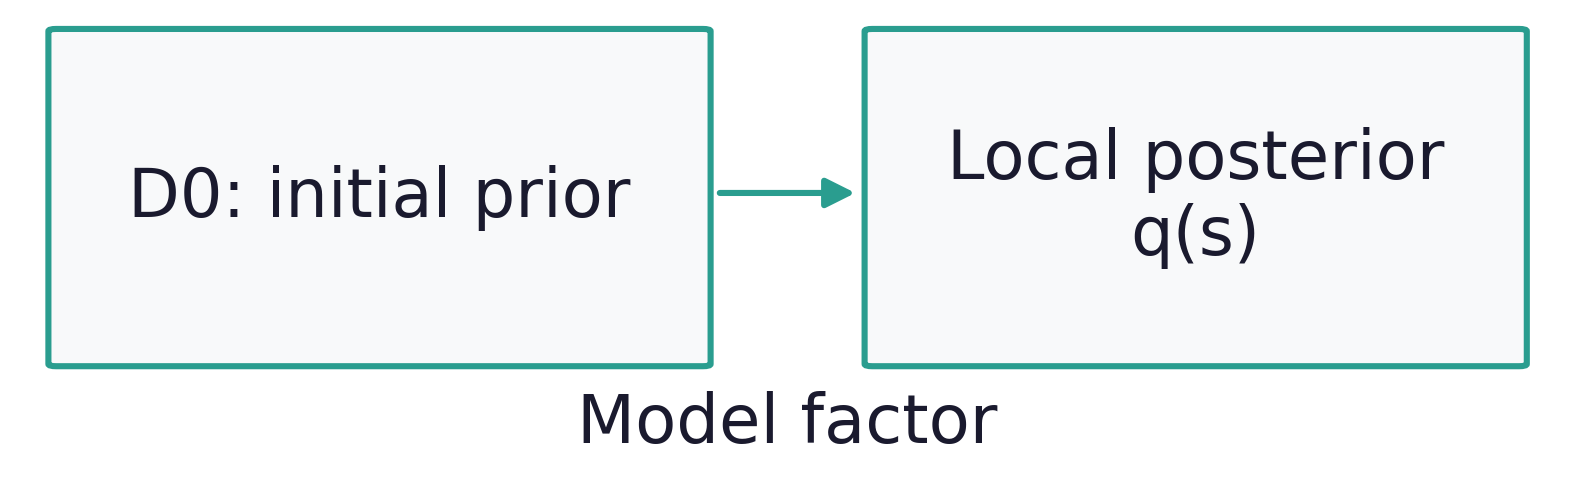
\includegraphics[keepaspectratio,width=0.98\linewidth,height=0.8\textheight,alt={D0: initial prior → Local posterior q(s): Model factor; data\_dependency.}]{../figures/generative_model_schema.slide-prior.png}
\refstepcounter{figure}\label{fig:generative-model-schema-slide-panel-7}
\end{figure}
\end{frame}

\begin{frame}{Generative model (part 15)}
\begin{figure}
\centering
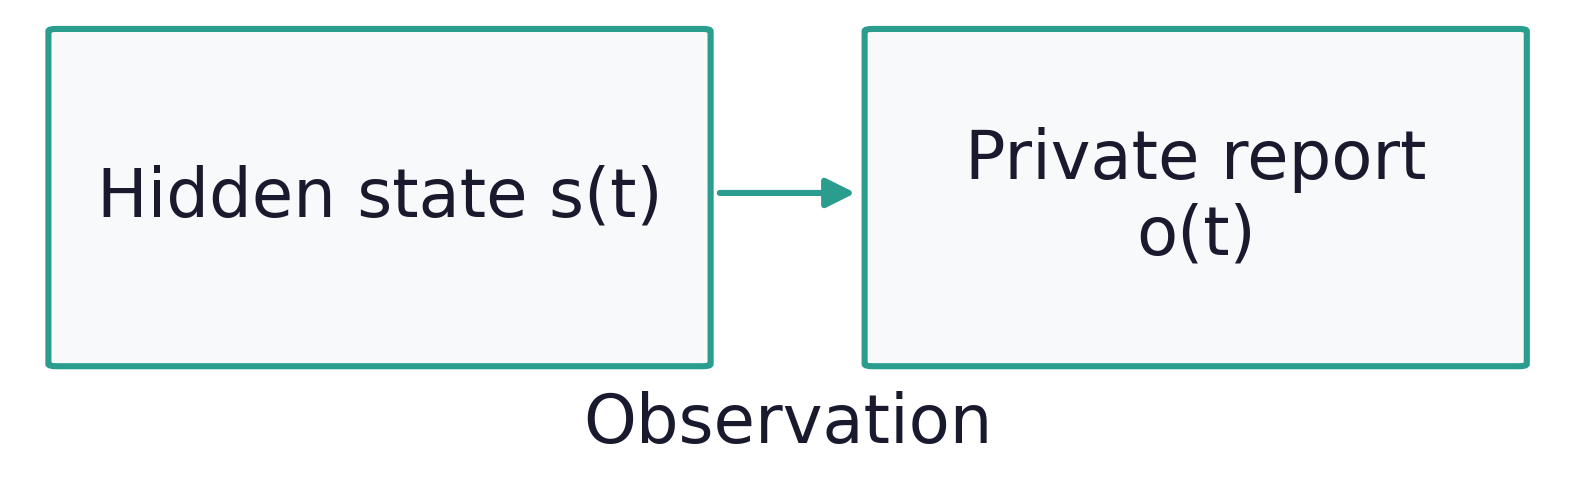
\includegraphics[keepaspectratio,width=0.98\linewidth,height=0.8\textheight,alt={Hidden state s(t) → Private report o(t): Observation; data\_dependency.}]{../figures/generative_model_schema.slide-time-sensing.png}
\refstepcounter{figure}\label{fig:generative-model-schema-slide-panel-8}
\end{figure}
\end{frame}

\begin{frame}{Generative model (part 16)}
\begin{figure}
\centering
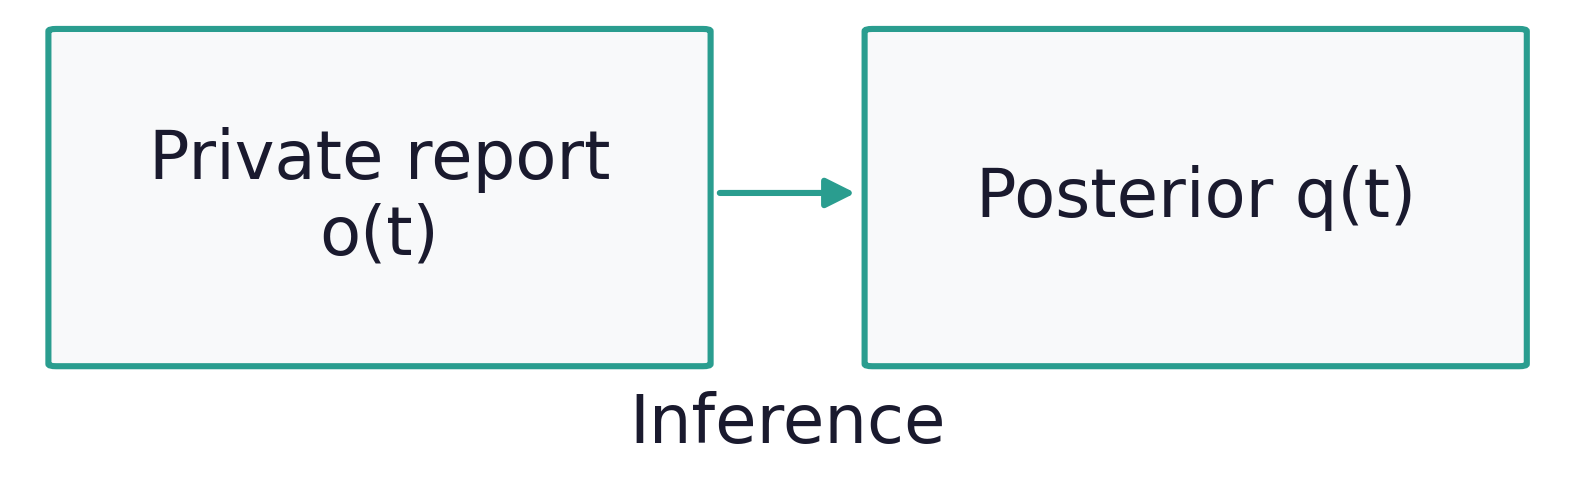
\includegraphics[keepaspectratio,width=0.98\linewidth,height=0.8\textheight,alt={Private report o(t) → Posterior q(t): Inference; data\_dependency.}]{../figures/generative_model_schema.slide-time-inference.png}
\refstepcounter{figure}\label{fig:generative-model-schema-slide-panel-9}
\end{figure}
\end{frame}

\begin{frame}{Generative model (part 17)}
\begin{figure}
\centering
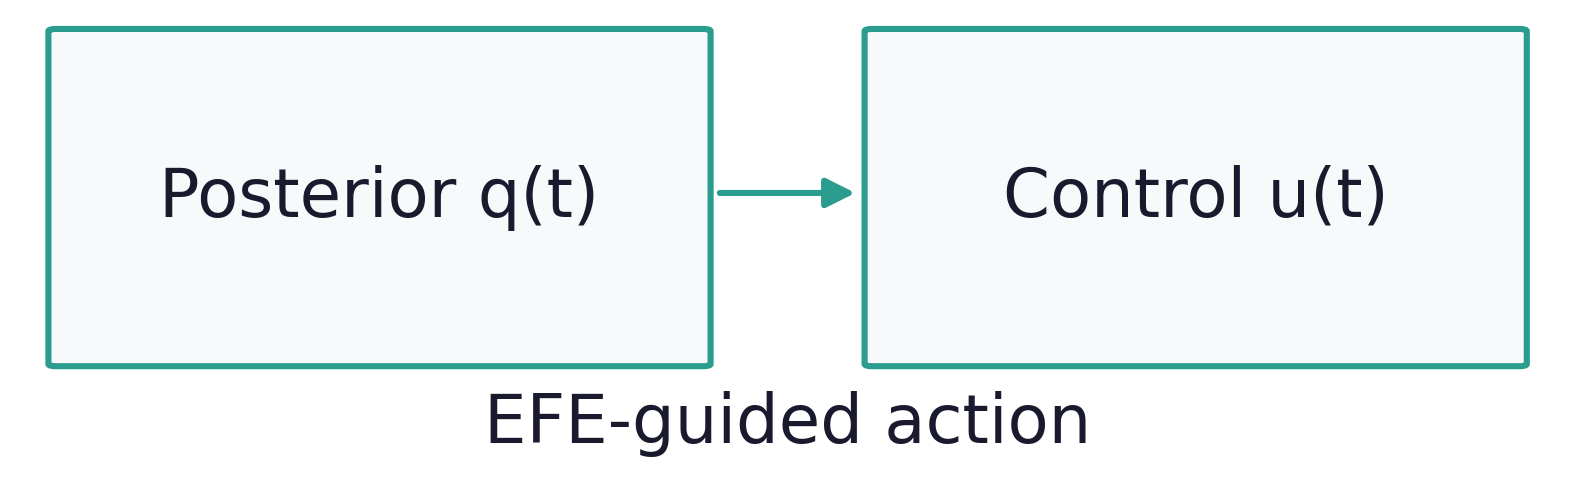
\includegraphics[keepaspectratio,width=0.98\linewidth,height=0.8\textheight,alt={Posterior q(t) → Control u(t): EFE-guided action; data\_dependency.}]{../figures/generative_model_schema.slide-time-control.png}
\refstepcounter{figure}\label{fig:generative-model-schema-slide-panel-10}
\end{figure}
\end{frame}

\begin{frame}{Generative model (part 18)}
\begin{figure}
\centering
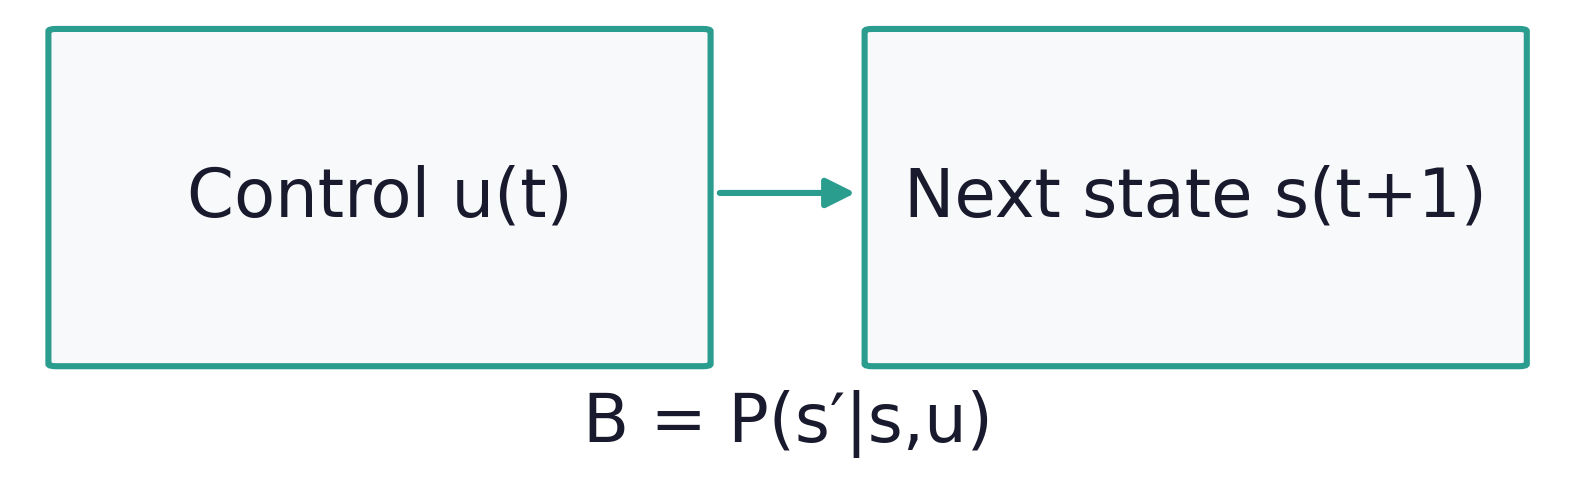
\includegraphics[keepaspectratio,width=0.98\linewidth,height=0.8\textheight,alt={Control u(t) → Next state s(t+1): B = P(s′\textbar s,u); data\_dependency.}]{../figures/generative_model_schema.slide-time-transition.png}
\refstepcounter{figure}\label{fig:generative-model-schema-slide-panel-11}
\end{figure}
\end{frame}

\begin{frame}{Generative model (part 19)}
\begin{figure}
\centering
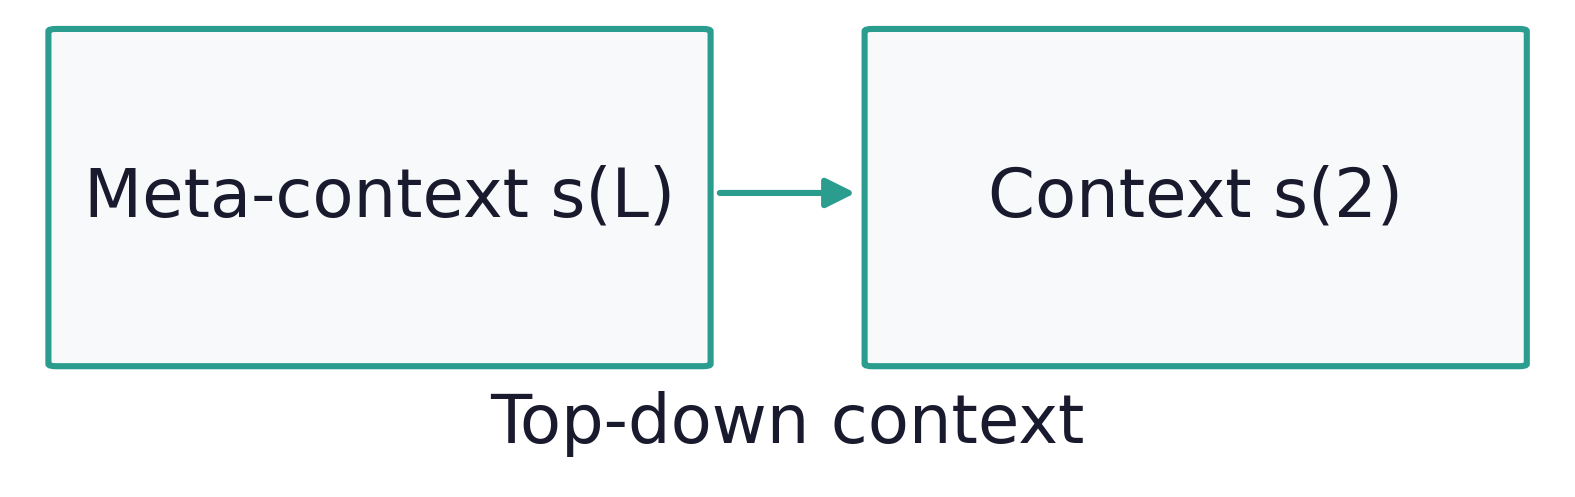
\includegraphics[keepaspectratio,width=0.98\linewidth,height=0.8\textheight,alt={Meta-context s(L) → Context s(2): Top-down context; data\_dependency.}]{../figures/generative_model_schema.slide-meta-context.png}
\refstepcounter{figure}\label{fig:generative-model-schema-slide-panel-12}
\end{figure}
\end{frame}

\begin{frame}{Generative model (part 20)}
\begin{figure}
\centering
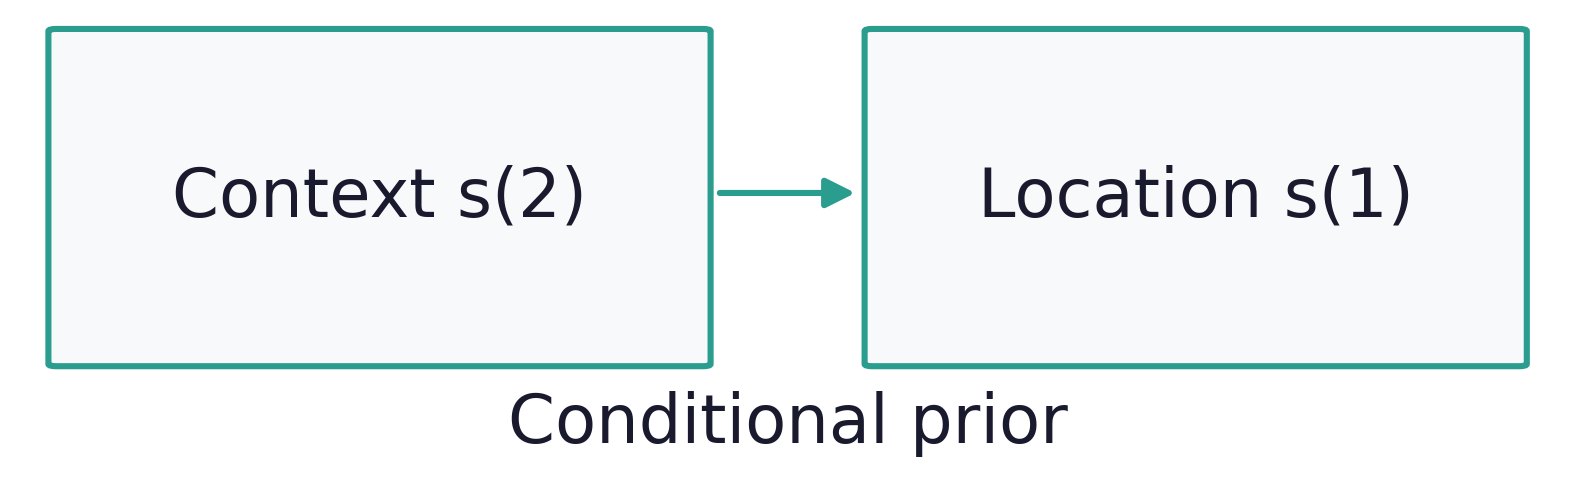
\includegraphics[keepaspectratio,width=0.98\linewidth,height=0.8\textheight,alt={Context s(2) → Location s(1): Conditional prior; data\_dependency.}]{../figures/generative_model_schema.slide-context-location.png}
\refstepcounter{figure}\label{fig:generative-model-schema-slide-panel-13}
\end{figure}
\end{frame}

\begin{frame}{Generative model (part 21)}
\begin{figure}
\centering
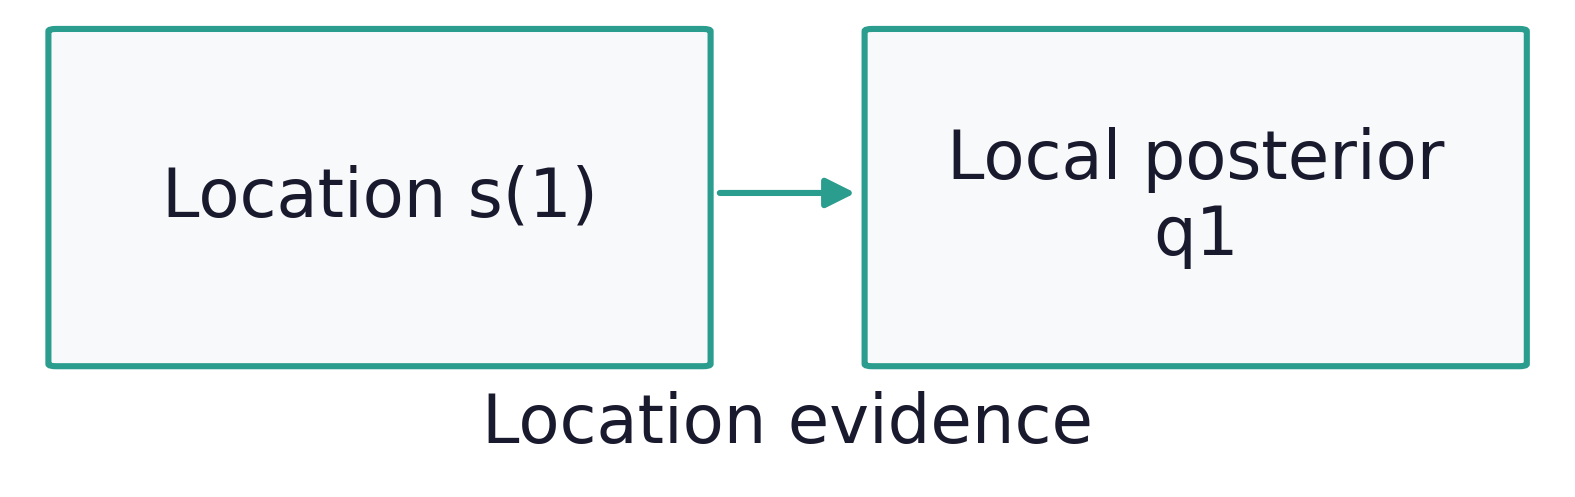
\includegraphics[keepaspectratio,width=0.98\linewidth,height=0.8\textheight,alt={Location s(1) → Local posterior q1: Location evidence; data\_dependency.}]{../figures/generative_model_schema.slide-location-posterior.png}
\refstepcounter{figure}\label{fig:generative-model-schema-slide-panel-14}
\end{figure}
\end{frame}

\begin{frame}{Generative model (part 22)}
\begin{figure}
\centering
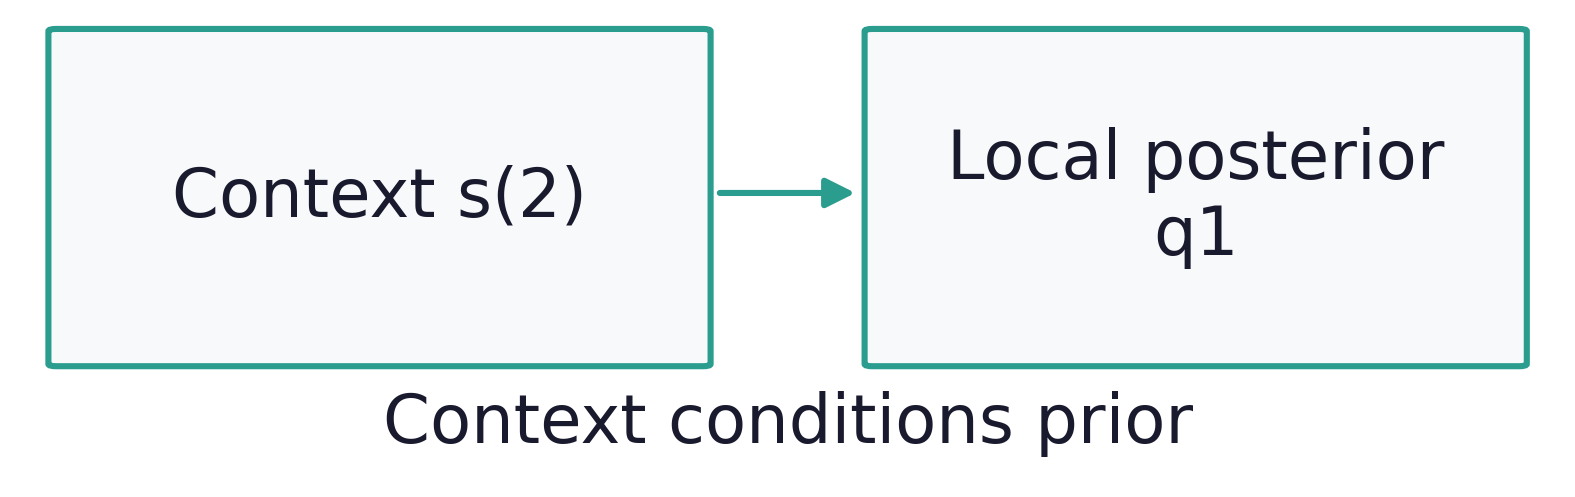
\includegraphics[keepaspectratio,width=0.98\linewidth,height=0.8\textheight,alt={Context s(2) → Local posterior q1: Context conditions prior; data\_dependency.}]{../figures/generative_model_schema.slide-context-posterior.png}
\refstepcounter{figure}\label{fig:generative-model-schema-slide-panel-15}
\end{figure}
\end{frame}

\begin{frame}{Generative model (part 23)}
\begin{figure}
\centering
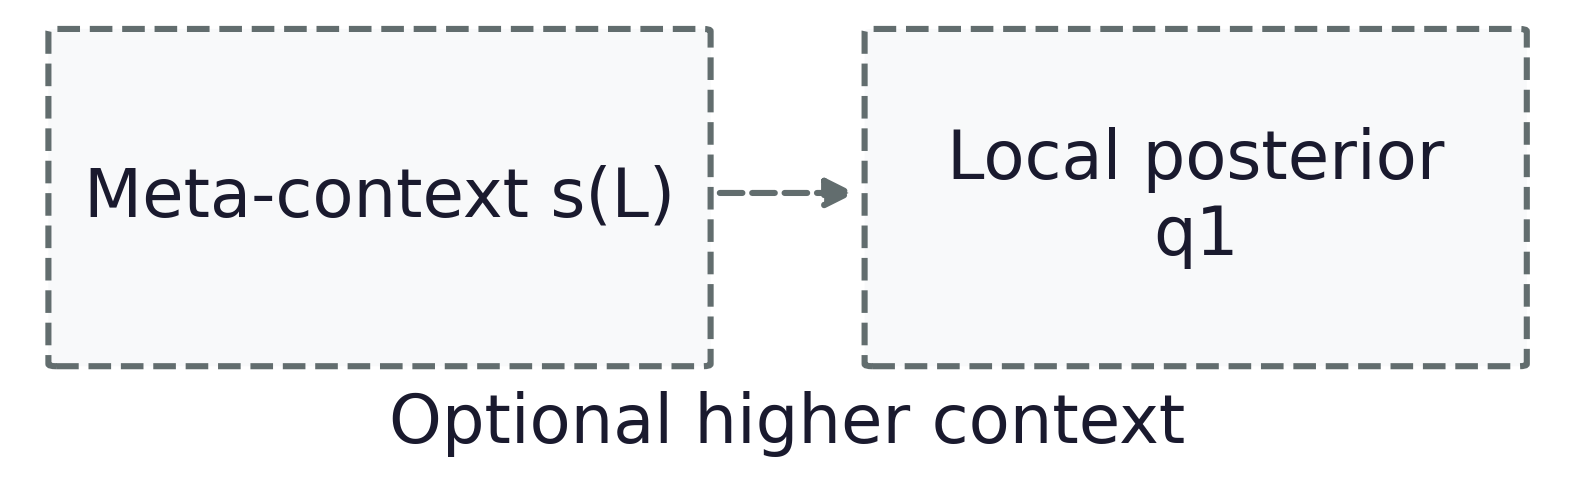
\includegraphics[keepaspectratio,width=0.98\linewidth,height=0.8\textheight,alt={Meta-context s(L) → Local posterior q1: Optional higher context; retained\_warning.}]{../figures/generative_model_schema.slide-meta-posterior.png}
\refstepcounter{figure}\label{fig:generative-model-schema-slide-panel-16}
\end{figure}
\end{frame}

\begin{frame}{Generative model (part 24)}
\begin{figure}
\centering
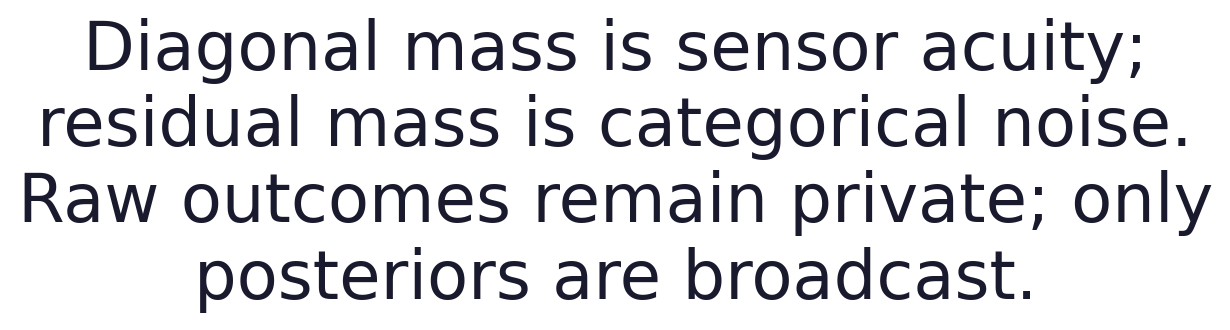
\includegraphics[keepaspectratio,width=0.98\linewidth,height=0.8\textheight,alt={Diagonal mass is sensor acuity; residual mass is categorical noise. Raw outcomes remain private; only posteriors are broadcast.}]{../figures/generative_model_schema.slide-sensor-key.png}
\refstepcounter{figure}\label{fig:generative-model-schema-slide-panel-17}
\end{figure}
\end{frame}

\begin{frame}{Generative model (part 25)}
\begin{figure}
\centering
\includegraphics[keepaspectratio,width=0.98\linewidth,height=0.8\textheight,alt={\$q(s)=\textbackslash mathrm\{softmax\}(\textbackslash ln D\_0+\textbackslash ln A{[}o,\textbackslash cdot{]})\$}]{../figures/generative_model_schema.slide-local-equation.png}
\refstepcounter{figure}\label{fig:generative-model-schema-slide-panel-18}
\end{figure}
\end{frame}

\begin{frame}{Generative model (part 26)}
\begin{figure}
\centering
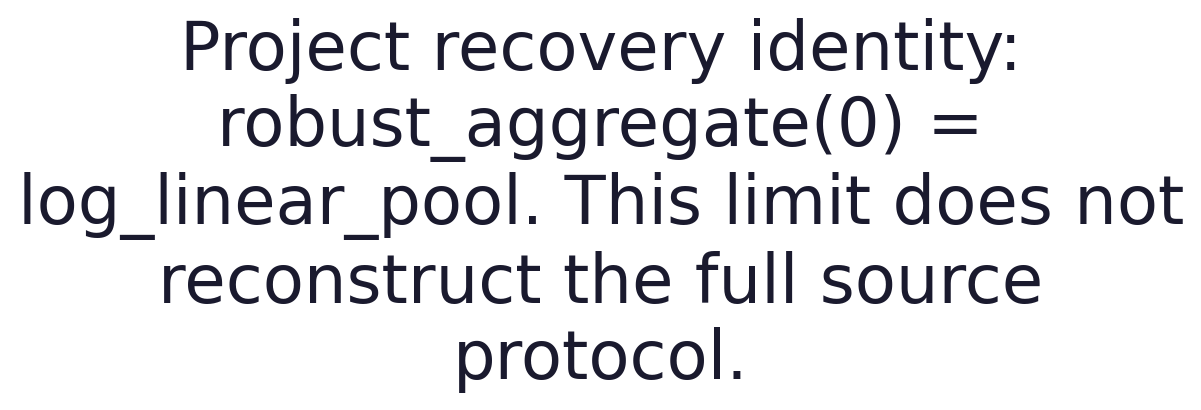
\includegraphics[keepaspectratio,width=0.98\linewidth,height=0.8\textheight,alt={Project recovery identity: robust\_aggregate(0) = log\_linear\_pool. This limit does not reconstruct the full source protocol.}]{../figures/generative_model_schema.slide-recovery.png}
\refstepcounter{figure}\label{fig:generative-model-schema-slide-panel-19}
\end{figure}
\end{frame}

\begin{frame}{Generative model (part 27)}
\begin{figure}
\centering
\includegraphics[keepaspectratio,width=0.98\linewidth,height=0.8\textheight,alt={\$\textbackslash bar q\_1=\textbackslash sum\_kq\_2{[}k{]}D\_\{1\textbar k\}\$}]{../figures/generative_model_schema.slide-mixture-equation.png}
\refstepcounter{figure}\label{fig:generative-model-schema-slide-panel-20}
\end{figure}
\end{frame}

\begin{frame}{Generative model (part 28)}
\begin{figure}
\centering
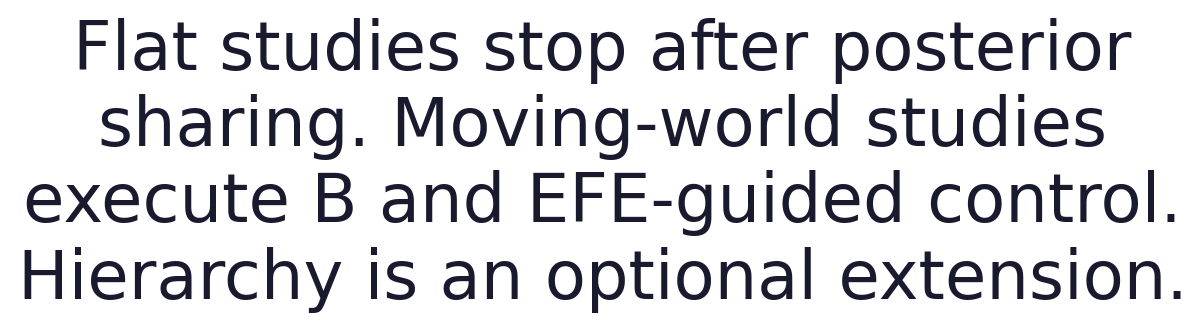
\includegraphics[keepaspectratio,width=0.98\linewidth,height=0.8\textheight,alt={Flat studies stop after posterior sharing. Moving-world studies execute B and EFE-guided control. Hierarchy is an optional extension.}]{../figures/generative_model_schema.slide-optional.png}
\refstepcounter{figure}\label{fig:generative-model-schema-slide-panel-21}
\end{figure}
\end{frame}

\begin{frame}{Generative model (part 29)}
\begin{figure}
\centering
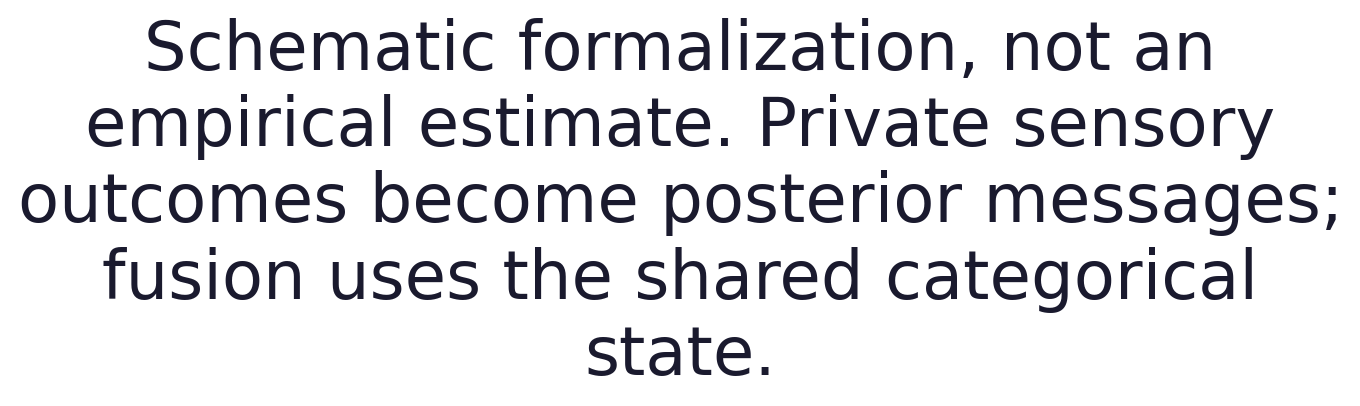
\includegraphics[keepaspectratio,width=0.98\linewidth,height=0.8\textheight,alt={Schematic formalization, not an empirical estimate. Private sensory outcomes become posterior messages; fusion uses the shared categorical state.}]{../figures/generative_model_schema.slide-scope.png}
\refstepcounter{figure}\label{fig:generative-model-schema-slide-panel-22}
\end{figure}
\end{frame}

\begin{frame}[fragile]{State space: one shared latent factor}
\protect\phantomsection\label{sec:methods-state-space}
The world holds one hidden factor: the creature's location on a square
grid of side \(L\), giving \(n_s = L^2\) location states. Our sentinel
world uses the \(3\times 3\) cardinality illustrated in Friston et al.
(2024), Fig. 1, so \(n_s = 9\) --- the cardinality
\texttt{pomdp.N\_LOCATIONS} exposes and \texttt{experiment\_config}
carries as \texttt{n\_locations}.
\end{frame}

\begin{frame}{State space: one shared\ldots{} (part 2)}
This single location factor is precisely the latent the colony gossips
about: it is the shared argument of the log-linear pool
(eq.~9) and of every belief-sharing round
(eq.~14). Fixing one hidden factor keeps the recovery
limits of sec.~6 closed-form and exactly testable,
\end{frame}

\begin{frame}{State space: one shared\ldots{} (part 3)}
rather than approximated.
\end{frame}

\begin{frame}{Four categorical tensors: likelihood, transitions,
preferences, priors}
\protect\phantomsection\label{sec:methods-abcd}
The generative model is the tuple \((A, B, C, D_0)\) in the discrete
active-inference convention: a categorical probability mass function is
a non-negative vector summing to one,
\end{frame}

\begin{frame}{Four categorical tensors (part 2)}
and a likelihood matrix is shape \((n_o, n_s)\) whose columns (indexed
by hidden state) are categorical.
\end{frame}

\begin{frame}[fragile]{Four categorical tensors (part 3)}
\textbf{Observation likelihood \(A = P(o\mid s)\).} Each sentinel
observes the creature's cell through a noisy sensor. With probability
\texttt{acuity} the sensor reports the true cell; the residual mass
\(1-\text{acuity}\) spreads uniformly over the other \(n_s-1\) cells.
With outcome cardinality \(n_o = n_s\),
\end{frame}

\begin{frame}{Four categorical tensors (part 4)}
the single location modality is one \((n_s, n_s)\) matrix:
\end{frame}

\begin{frame}{Four categorical tensors (part 5)}
\begin{equation}\tag{15}\protect\phantomsection\label{eq:observation-likelihood}{
\begin{aligned}
A_{o s} &= \text{acuity}
&& \text{if }o=s,\\
A_{o s} &= \frac{1-\text{acuity}}{n_s-1}
&& \text{if }o\neq s,\\
\sum_o A_{o s} &= 1.
\end{aligned}
}\end{equation}
\end{frame}

\begin{frame}{Four categorical tensors (part 6)}
The acuity in eq.~15 tunes how peaked the
sensor is: high acuity gives a near-diagonal \(A\) that pins the
creature; the belief-sharing study deliberately runs the colony at the
low acuity \(\text{acuity} = 0.55\), where no single sentinel can
resolve the location alone and the colony must pool evidence to do so.
\end{frame}

\begin{frame}{Four categorical tensors (part 7)}
When a seeded generator is supplied, each sentinel's acuity is jittered
by a small non-negative perturbation, so a colony carries slightly
heterogeneous likelihoods while every column remains a proper pmf.
\end{frame}

\begin{frame}[fragile]{Four categorical tensors (part 8)}
\textbf{Transition tensor \(B = P(s'\mid s, u)\).} The creature moves on
the grid under three control paths --- \texttt{still}, \texttt{left},
\texttt{right} --- so \(B\) has shape \((n_s, n_s, n_u)\) with
\(n_u = 3\). \texttt{still} is the deterministic self-loop;
\texttt{left} and \texttt{right} decrement and increment the grid
column,
\end{frame}

\begin{frame}{Four categorical tensors (part 9)}
saturating at the walls (a wall-adjacent move in the wall's direction is
a self-loop).
\end{frame}

\begin{frame}{Four categorical tensors (part 10)}
All three controls act on the column index alone, so the creature's row
is preserved and its motion is confined to the horizontal axis of the
grid --- a deliberate one-dimensional control over the two-dimensional
location factor. Every slice \(B_{\cdot\,\cdot\,u}\) is
column-normalized by construction,
\end{frame}

\begin{frame}{Four categorical tensors (part 11)}
so the transition is a valid categorical for each action.
\end{frame}

\begin{frame}{Four categorical tensors (part 12)}
\textbf{Log-preference \(C\).} The sentinel prefers to \emph{see} the
creature near the den (the center cell), encoded as a log-preference
vector of shape \((n_o, 1)\) with a positive bump on the center outcome
and zero elsewhere.
\end{frame}

\begin{frame}{Four categorical tensors (part 13)}
The preferred-outcome distribution that the expected-free-energy
decomposition of sec.~5.15 uses is
\(p_C(o) = \mathrm{softmax}(C)[o]\).
\end{frame}

\begin{frame}{Four categorical tensors (part 14)}
\textbf{Initial prior \(D_0\).} The creature is believed to start at the
grid center, so \(D_0\) of shape \((n_s, 1)\) places unit mass on the
center cell. \(D_0\) enters state inference as the log-prior of the
one-step variational update (eq.~16 below).
\end{frame}

\begin{frame}{Four categorical tensors (part 15)}
The columns-are-pmfs invariant is not assumed --- it is pinned by
ISC-15, which checks that every column of \(A\) and of each
\(B_{\cdot\,\cdot\,u}\) sums to one.
\end{frame}

\begin{frame}{One-step variational state inference in the grid world}
\protect\phantomsection\label{sec:methods-state-inference}
Given an observation \(o\), a sentinel forms a posterior over the
creature's location by a single softmax step (Friston et al. (2024), Eq.
4): the log-prior plus the additive log-likelihood message,
\end{frame}

\begin{frame}{One-step variational state\ldots{} (part 2)}
summed over any conditionally independent modalities \(m\),
\end{frame}

\begin{frame}{One-step variational state\ldots{} (part 3)}
\begin{equation}\tag{16}\protect\phantomsection\label{eq:state-inference}{
q(s)
= \mathrm{softmax}\!\left(
\begin{aligned}
&\ln D_0(s)\\
&\quad + \textstyle\sum_m \ln A_m[o_m, s]
\end{aligned}
\right).
}\end{equation}
\end{frame}

\begin{frame}{One-step variational state\ldots{} (part 4)}
The message \(\ln A_m[o_m, \cdot]\) is the row of \(A_m\) that the
observed outcome selects; summing messages over modalities makes each
modality an additive evidence term --- the categorical
product-of-experts. The companion variational free energy, the scalar
eq.~16 minimizes, is
\end{frame}

\begin{frame}{One-step variational state\ldots{} (part 5)}
\begin{equation}\tag{17}\protect\phantomsection\label{eq:variational-free-energy}{
\begin{aligned}
F[q]
&= \mathbb{E}_q\!\left[
\begin{aligned}
&\ln q(s) - \ln D_0(s)\\
&\quad - \textstyle\sum_m \ln A_m[o_m, s]
\end{aligned}
\right]\\
&= \mathrm{KL}\big(q \,\|\, D_0\big)
   - \mathbb{E}_q\!\big[\textstyle\sum_m \ln A_m[o_m, s]\big].
\end{aligned}
}\end{equation}
\end{frame}

\begin{frame}{One-step variational state\ldots{} (part 6)}
reported in nats. The one-step posterior of eq.~16
is its unique minimizer, where \(F\) equals the negative log model
evidence.
\end{frame}

\begin{frame}[fragile]{One-step variational state\ldots{} (part 7)}
Both live in \texttt{belief\_updating.infer\_states} and
\texttt{belief\_updating.vfe}, and the free energy of
eq.~17 is the quantity the
communicating-versus-incommunicado colony comparison of
sec.~5.22 scores.
\end{frame}

\begin{frame}{One-step variational state\ldots{} (part 8)}
This inference step is not a separate mechanism bolted onto the colony:
it is the \(L=\mathrm{NLL}\), learning-rate-1 special case of the
generalized-Bayes posterior eq.~2, reusing the same
locked softmax.
\end{frame}

\begin{frame}{One-step variational state\ldots{} (part 9)}
That client identity recovers the stated categorical Bayes substrate at
its trusting limits. The separate server identity in
sec.~5.8 then yields the project log-linear
pool under its qualified Eq. 7 message-combination bridge;
\end{frame}

\begin{frame}{One-step variational state\ldots{} (part 10)}
together these do not recover the complete Friston protocol
(sec.~6).
\end{frame}

\begin{frame}{Hidden-state to action loop: the POMDP substrate}
\protect\phantomsection\label{sec:methods-pomdp-loop}
The categorical POMDP loop in fig.~5 separates the
common latent-state substrate from the federation transport. In the
sentinel interpretation, an agent is a location-sensitive observer:
\end{frame}

\begin{frame}{Hidden-state to action loop (part 2)}
the hidden state is one of 9 cells, the private outcome is a noisy
categorical report of that location, and the agent sends its posterior
over the location rather than the report itself.
\end{frame}

\begin{frame}{Hidden-state to action loop (part 3)}
The flat belief-sharing studies use the observation, posterior, and
communication subset; the moving-world extension also executes
transition and EFE-guided action paths.
\end{frame}

\begin{frame}{Hidden-state to action loop (part 4)}
The diagram therefore gives readers the active-inference context without
turning a conceptual loop into a claim that every study estimates every
latent or policy quantity.
\end{frame}

\begin{frame}{Hidden-state to action loop (part 5)}
\begin{figure}
\centering
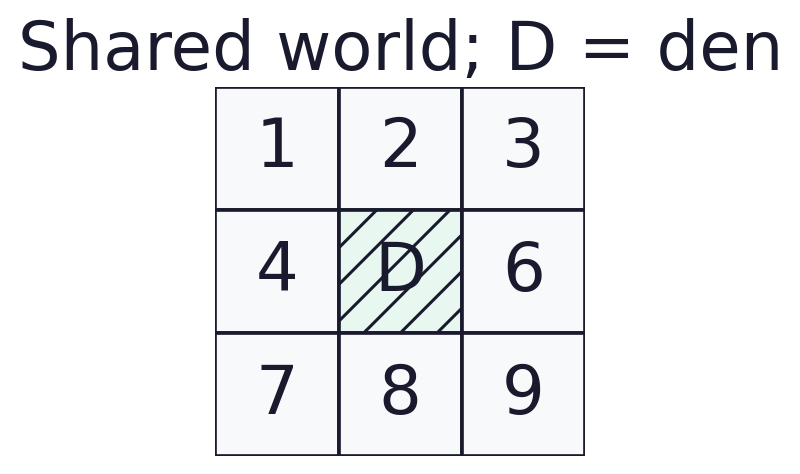
\includegraphics[keepaspectratio,width=0.98\linewidth,height=0.8\textheight,alt={Shared world; D = den: nine-cell topology; cell 5 is hatched. Schematic only, no measured probability scale.}]{../figures/pomdp_loop.slide-world.png}
\refstepcounter{figure}\label{fig:pomdp-loop-slide-panel-1}
\end{figure}
\end{frame}

\begin{frame}{Hidden-state to action loop (part 6)}
\begin{figure}
\centering
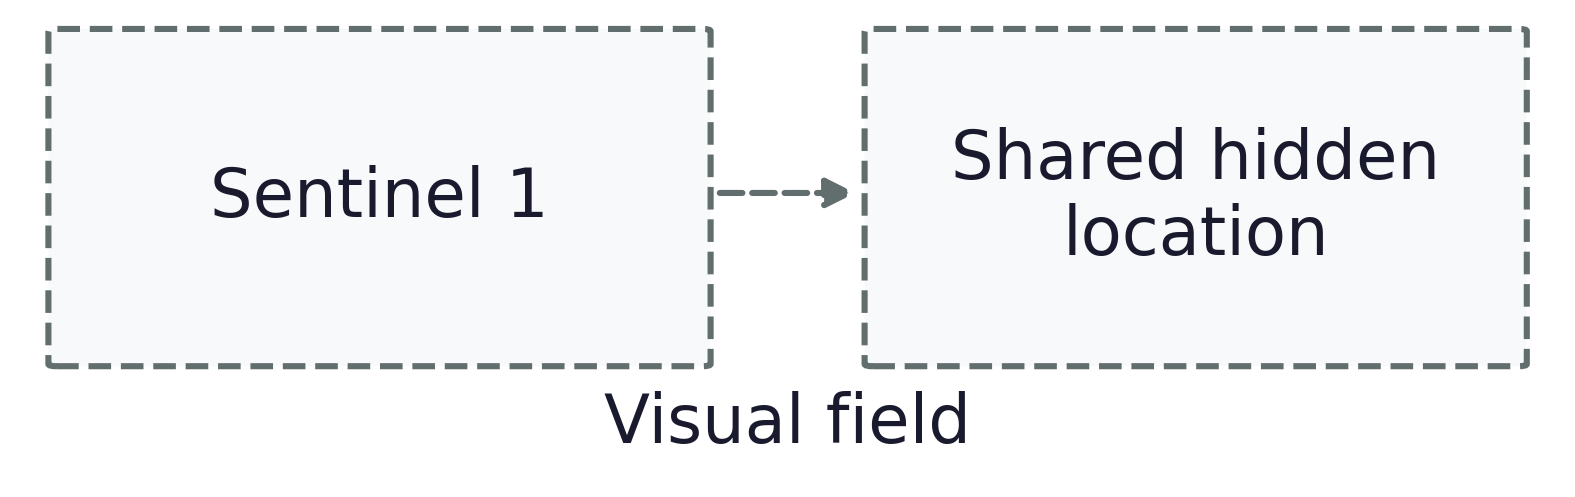
\includegraphics[keepaspectratio,width=0.98\linewidth,height=0.8\textheight,alt={Sentinel 1 → Shared hidden location: Visual field; retained\_warning.}]{../figures/pomdp_loop.slide-visual-field-1.png}
\refstepcounter{figure}\label{fig:pomdp-loop-slide-panel-2}
\end{figure}
\end{frame}

\begin{frame}{Hidden-state to action loop (part 7)}
\begin{figure}
\centering
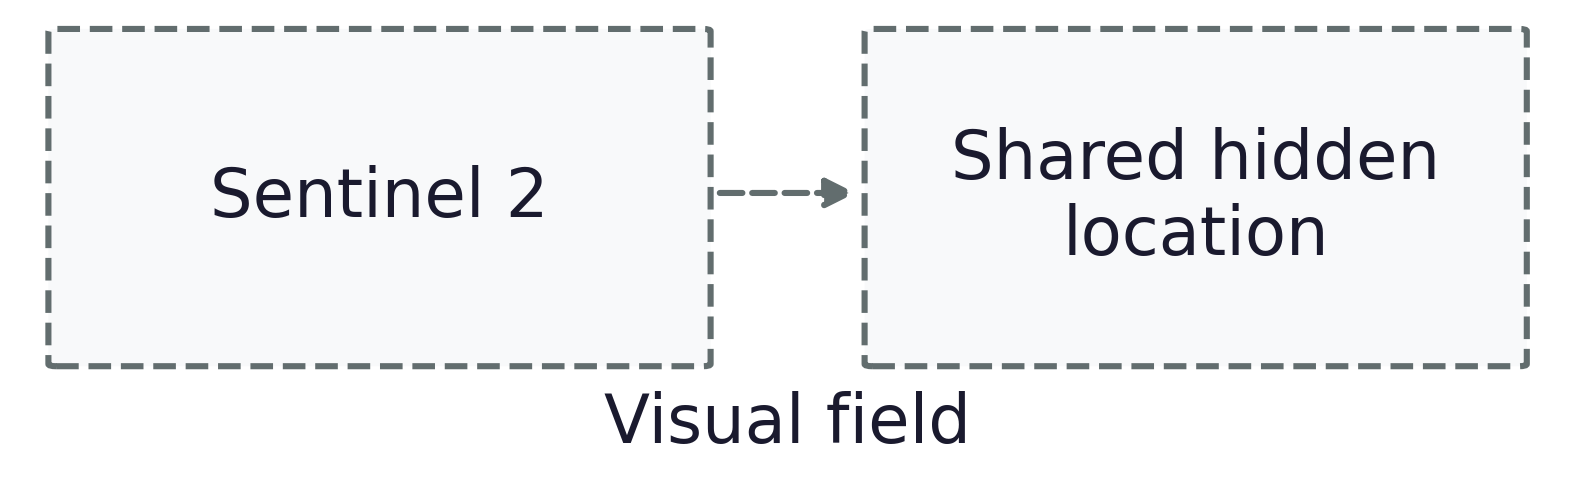
\includegraphics[keepaspectratio,width=0.98\linewidth,height=0.8\textheight,alt={Sentinel 2 → Shared hidden location: Visual field; retained\_warning.}]{../figures/pomdp_loop.slide-visual-field-2.png}
\refstepcounter{figure}\label{fig:pomdp-loop-slide-panel-3}
\end{figure}
\end{frame}

\begin{frame}{Hidden-state to action loop (part 8)}
\begin{figure}
\centering
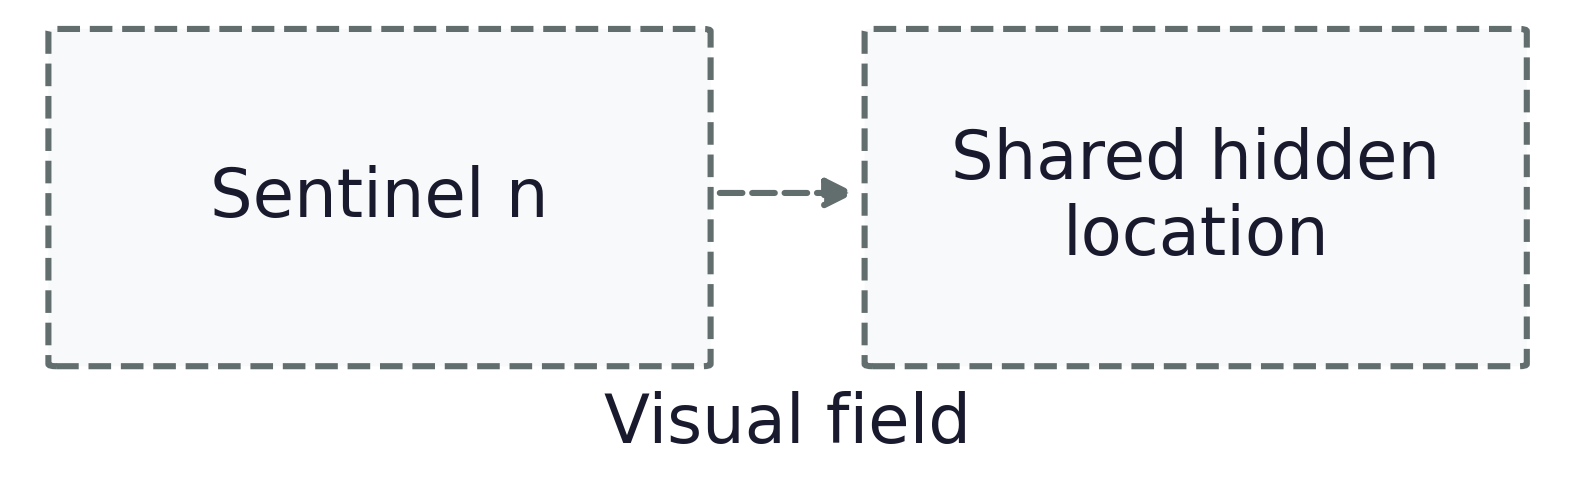
\includegraphics[keepaspectratio,width=0.98\linewidth,height=0.8\textheight,alt={Sentinel n → Shared hidden location: Visual field; retained\_warning.}]{../figures/pomdp_loop.slide-visual-field-n.png}
\refstepcounter{figure}\label{fig:pomdp-loop-slide-panel-4}
\end{figure}
\end{frame}

\begin{frame}{Hidden-state to action loop (part 9)}
\begin{figure}
\centering
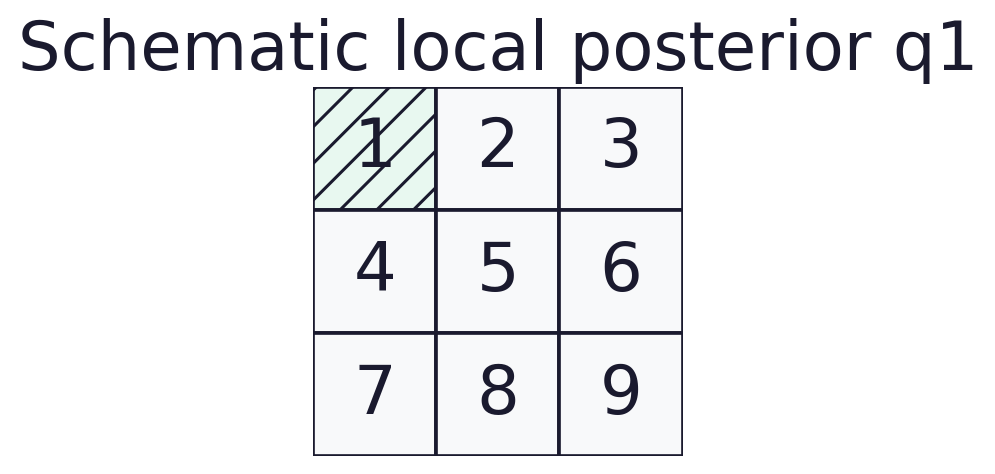
\includegraphics[keepaspectratio,width=0.98\linewidth,height=0.8\textheight,alt={Schematic local posterior q1: nine-cell topology; cell 1 is hatched. Schematic only, no measured probability scale.}]{../figures/pomdp_loop.slide-local-posterior-1.png}
\refstepcounter{figure}\label{fig:pomdp-loop-slide-panel-5}
\end{figure}
\end{frame}

\begin{frame}{Hidden-state to action loop (part 10)}
\begin{figure}
\centering
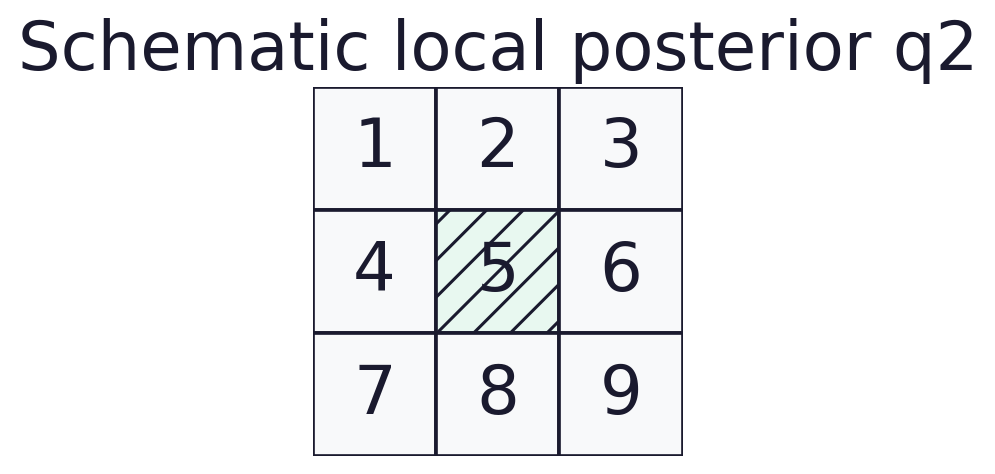
\includegraphics[keepaspectratio,width=0.98\linewidth,height=0.8\textheight,alt={Schematic local posterior q2: nine-cell topology; cell 5 is hatched. Schematic only, no measured probability scale.}]{../figures/pomdp_loop.slide-local-posterior-2.png}
\refstepcounter{figure}\label{fig:pomdp-loop-slide-panel-6}
\end{figure}
\end{frame}

\begin{frame}{Hidden-state to action loop (part 11)}
\begin{figure}
\centering
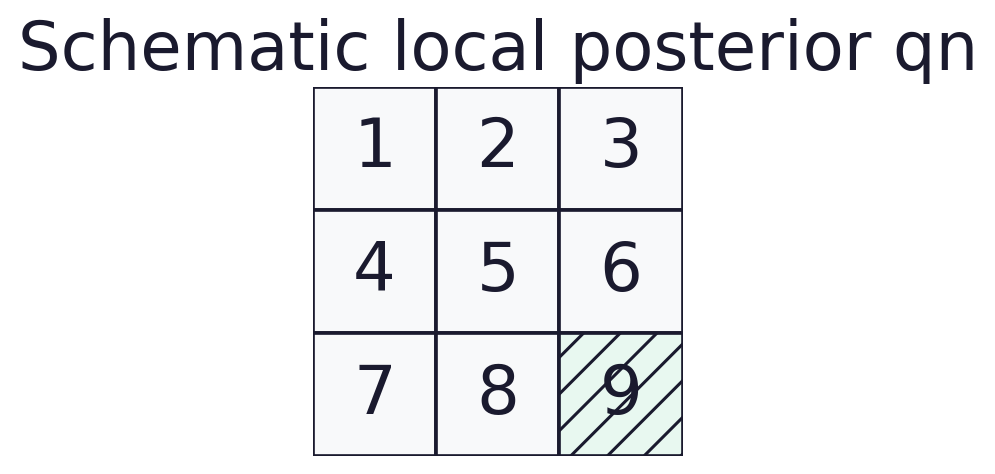
\includegraphics[keepaspectratio,width=0.98\linewidth,height=0.8\textheight,alt={Schematic local posterior qn: nine-cell topology; cell 9 is hatched. Schematic only, no measured probability scale.}]{../figures/pomdp_loop.slide-local-posterior-n.png}
\refstepcounter{figure}\label{fig:pomdp-loop-slide-panel-7}
\end{figure}
\end{frame}

\begin{frame}{Hidden-state to action loop (part 12)}
\begin{figure}
\centering
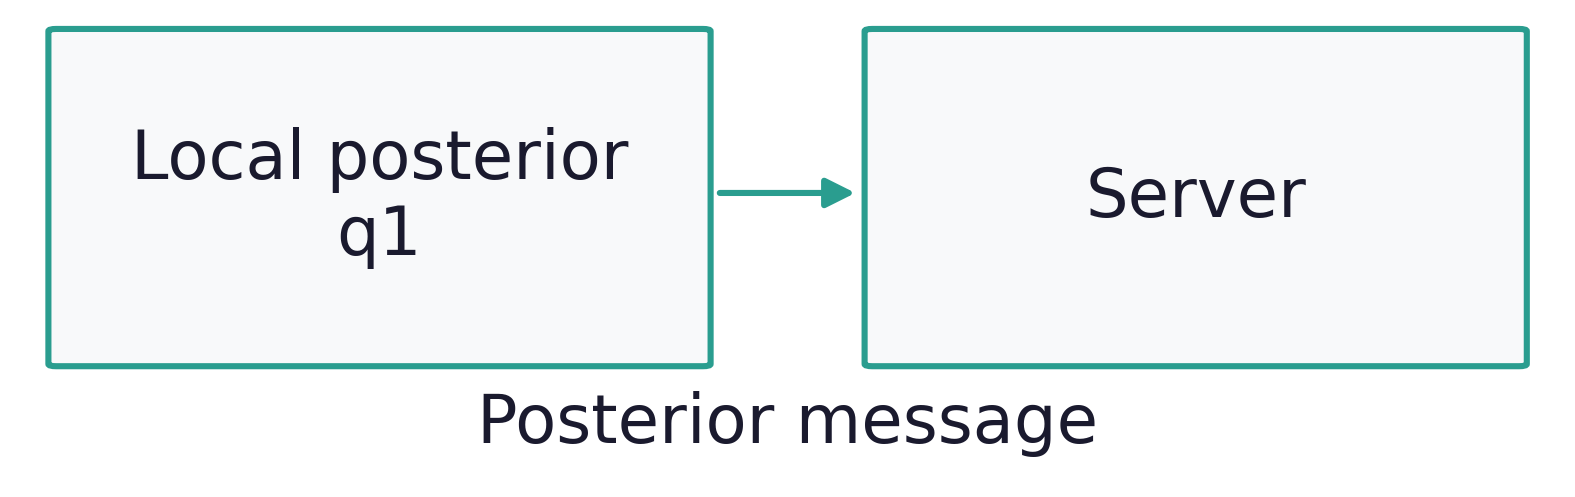
\includegraphics[keepaspectratio,width=0.98\linewidth,height=0.8\textheight,alt={Local posterior q1 → Server: Posterior message; data\_dependency.}]{../figures/pomdp_loop.slide-message-1.png}
\refstepcounter{figure}\label{fig:pomdp-loop-slide-panel-8}
\end{figure}
\end{frame}

\begin{frame}{Hidden-state to action loop (part 13)}
\begin{figure}
\centering
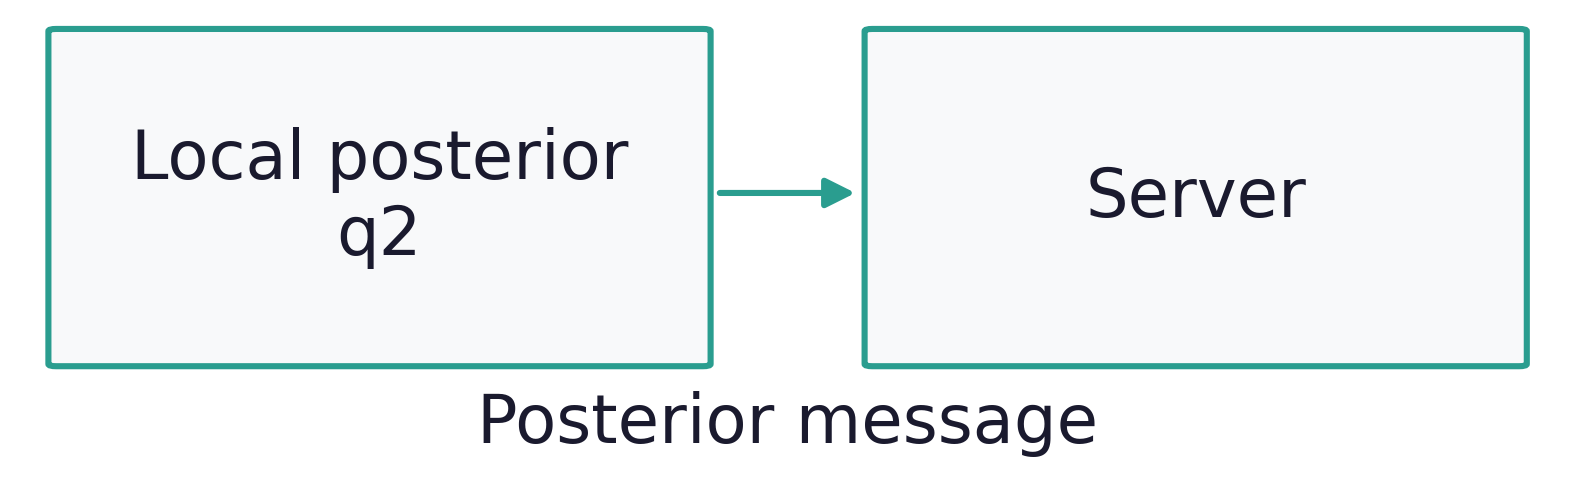
\includegraphics[keepaspectratio,width=0.98\linewidth,height=0.8\textheight,alt={Local posterior q2 → Server: Posterior message; data\_dependency.}]{../figures/pomdp_loop.slide-message-2.png}
\refstepcounter{figure}\label{fig:pomdp-loop-slide-panel-9}
\end{figure}
\end{frame}

\begin{frame}{Hidden-state to action loop (part 14)}
\begin{figure}
\centering
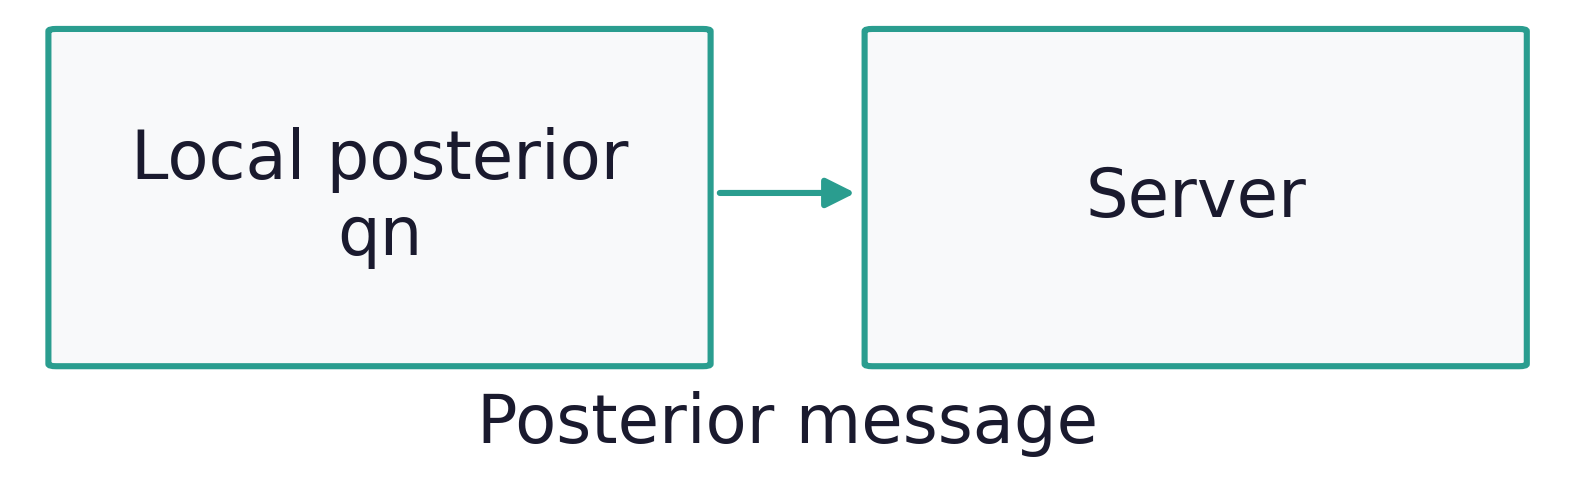
\includegraphics[keepaspectratio,width=0.98\linewidth,height=0.8\textheight,alt={Local posterior qn → Server: Posterior message; data\_dependency.}]{../figures/pomdp_loop.slide-message-n.png}
\refstepcounter{figure}\label{fig:pomdp-loop-slide-panel-10}
\end{figure}
\end{frame}

\begin{frame}{Hidden-state to action loop (part 15)}
\begin{figure}
\centering
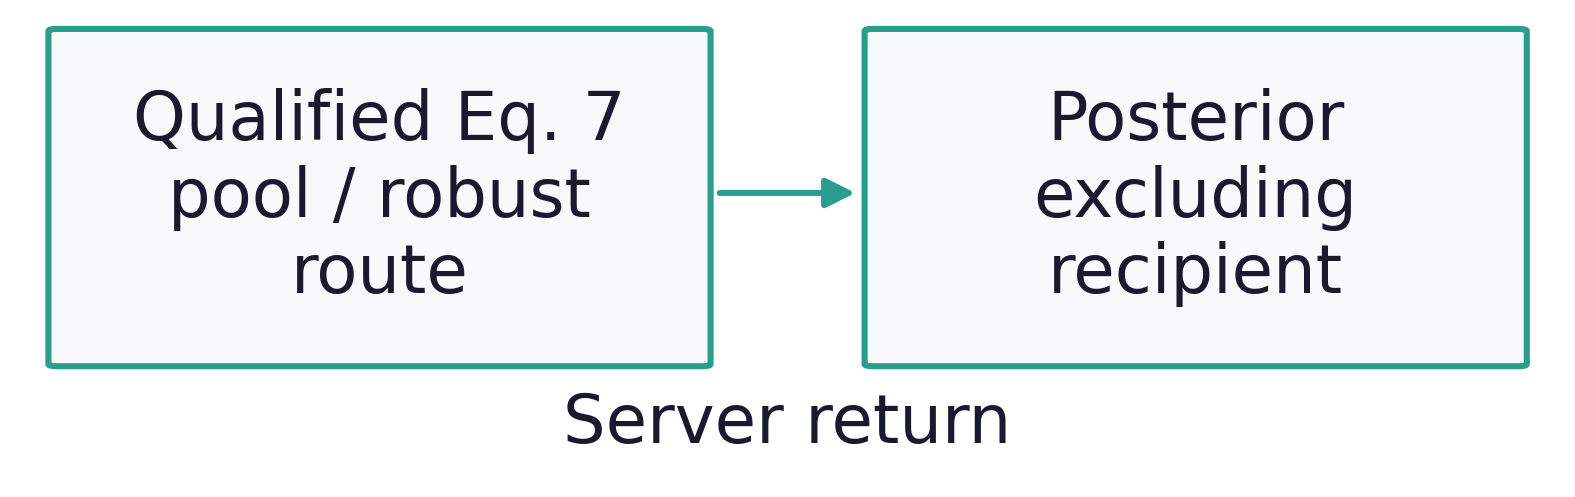
\includegraphics[keepaspectratio,width=0.98\linewidth,height=0.8\textheight,alt={Qualified Eq. 7 pool / robust route → Posterior excluding recipient: Server return; data\_dependency.}]{../figures/pomdp_loop.slide-return.png}
\refstepcounter{figure}\label{fig:pomdp-loop-slide-panel-11}
\end{figure}
\end{frame}

\begin{frame}{Hidden-state to action loop (part 16)}
\begin{figure}
\centering
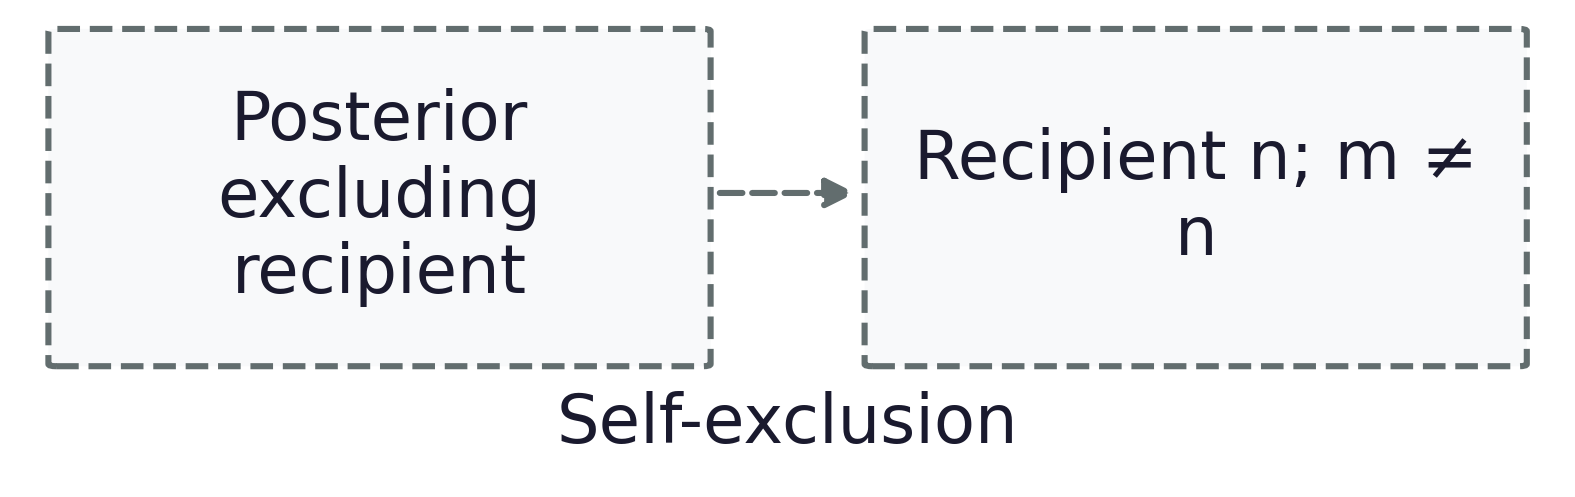
\includegraphics[keepaspectratio,width=0.98\linewidth,height=0.8\textheight,alt={Posterior excluding recipient → Recipient n; m ≠ n: Self-exclusion; retained\_warning.}]{../figures/pomdp_loop.slide-recipient.png}
\refstepcounter{figure}\label{fig:pomdp-loop-slide-panel-12}
\end{figure}
\end{frame}

\begin{frame}{Hidden-state to action loop (part 17)}
\begin{figure}
\centering
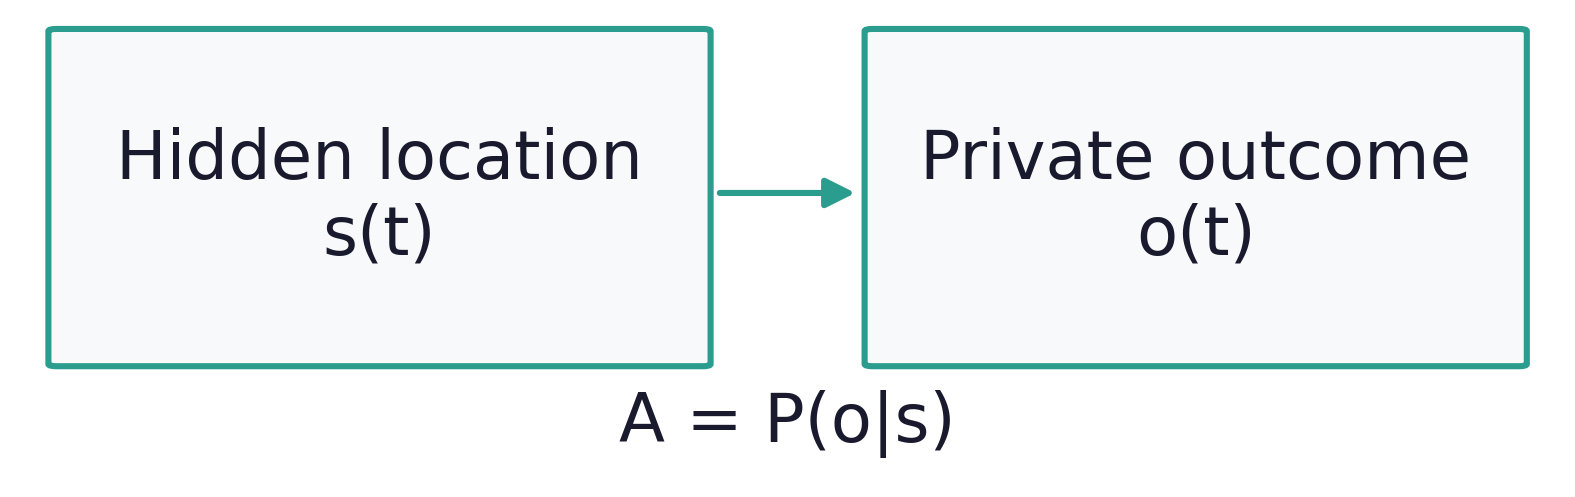
\includegraphics[keepaspectratio,width=0.98\linewidth,height=0.8\textheight,alt={Hidden location s(t) → Private outcome o(t): A = P(o\textbar s); data\_dependency.}]{../figures/pomdp_loop.slide-sensing.png}
\refstepcounter{figure}\label{fig:pomdp-loop-slide-panel-13}
\end{figure}
\end{frame}

\begin{frame}{Hidden-state to action loop (part 18)}
\begin{figure}
\centering
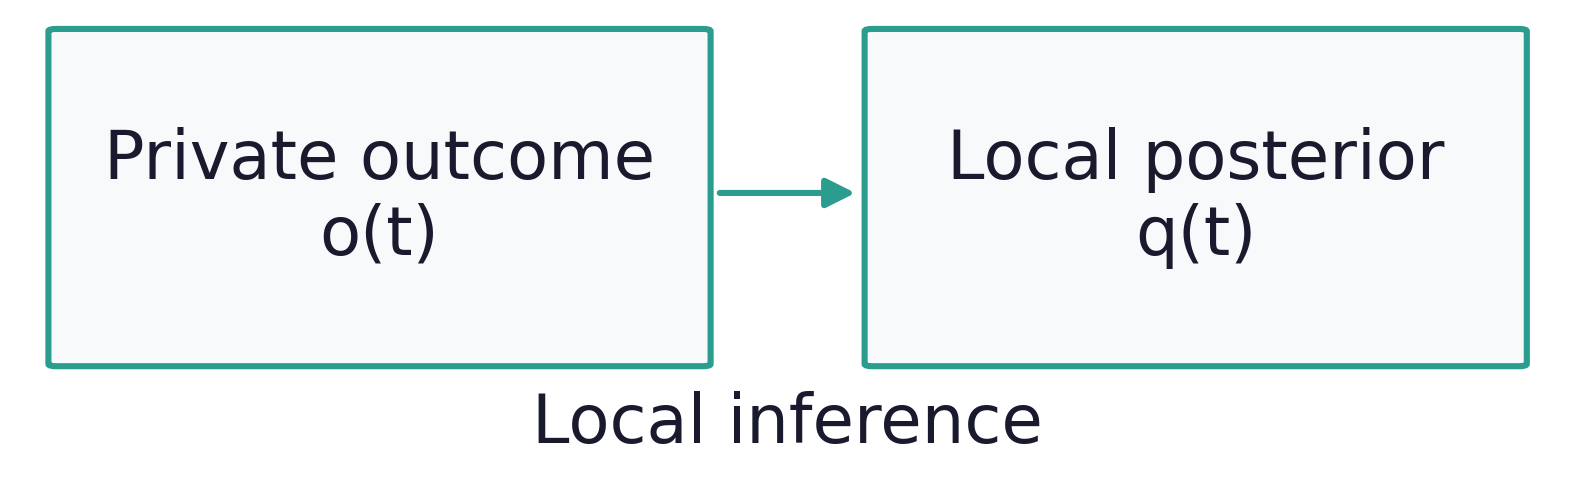
\includegraphics[keepaspectratio,width=0.98\linewidth,height=0.8\textheight,alt={Private outcome o(t) → Local posterior q(t): Local inference; data\_dependency.}]{../figures/pomdp_loop.slide-inference.png}
\refstepcounter{figure}\label{fig:pomdp-loop-slide-panel-14}
\end{figure}
\end{frame}

\begin{frame}{Hidden-state to action loop (part 19)}
\begin{figure}
\centering
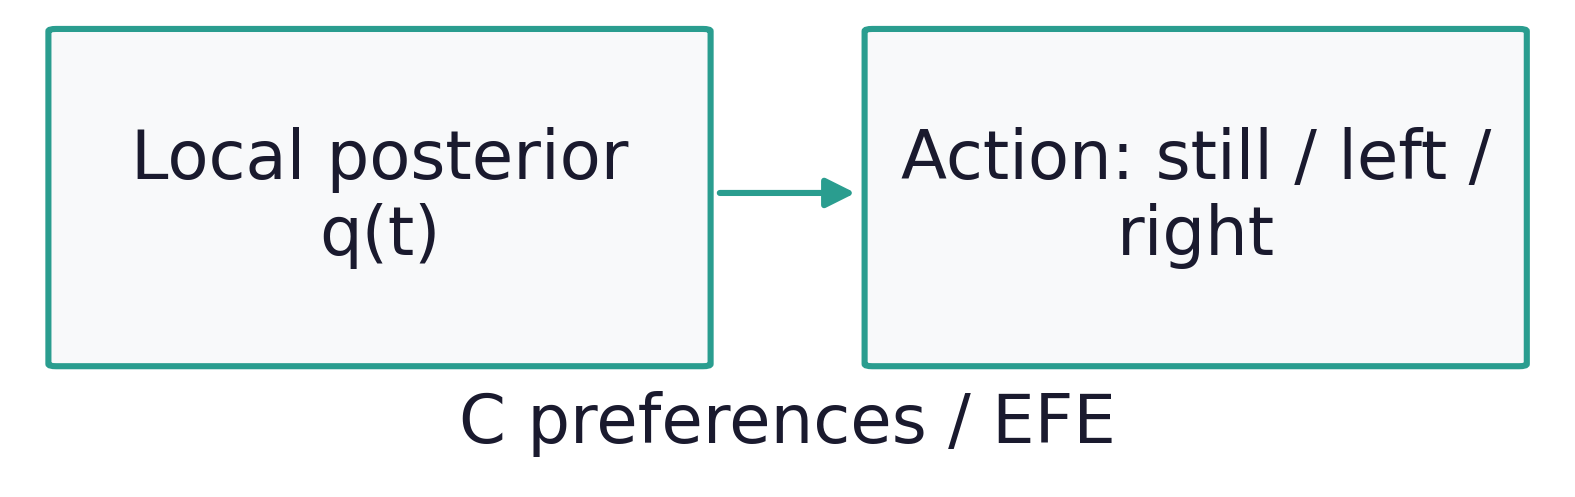
\includegraphics[keepaspectratio,width=0.98\linewidth,height=0.8\textheight,alt={Local posterior q(t) → Action: still / left / right: C preferences / EFE; data\_dependency.}]{../figures/pomdp_loop.slide-policy.png}
\refstepcounter{figure}\label{fig:pomdp-loop-slide-panel-15}
\end{figure}
\end{frame}

\begin{frame}{Hidden-state to action loop (part 20)}
\begin{figure}
\centering
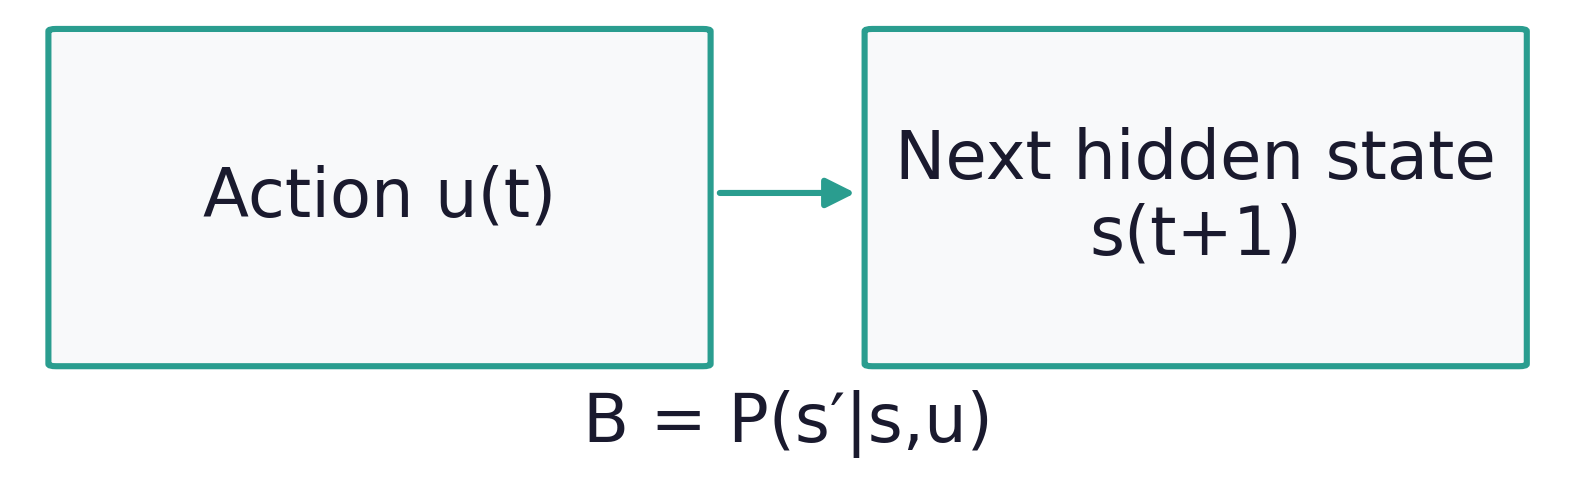
\includegraphics[keepaspectratio,width=0.98\linewidth,height=0.8\textheight,alt={Action u(t) → Next hidden state s(t+1): B = P(s′\textbar s,u); data\_dependency.}]{../figures/pomdp_loop.slide-transition.png}
\refstepcounter{figure}\label{fig:pomdp-loop-slide-panel-16}
\end{figure}
\end{frame}

\begin{frame}{Hidden-state to action loop (part 21)}
\begin{figure}
\centering
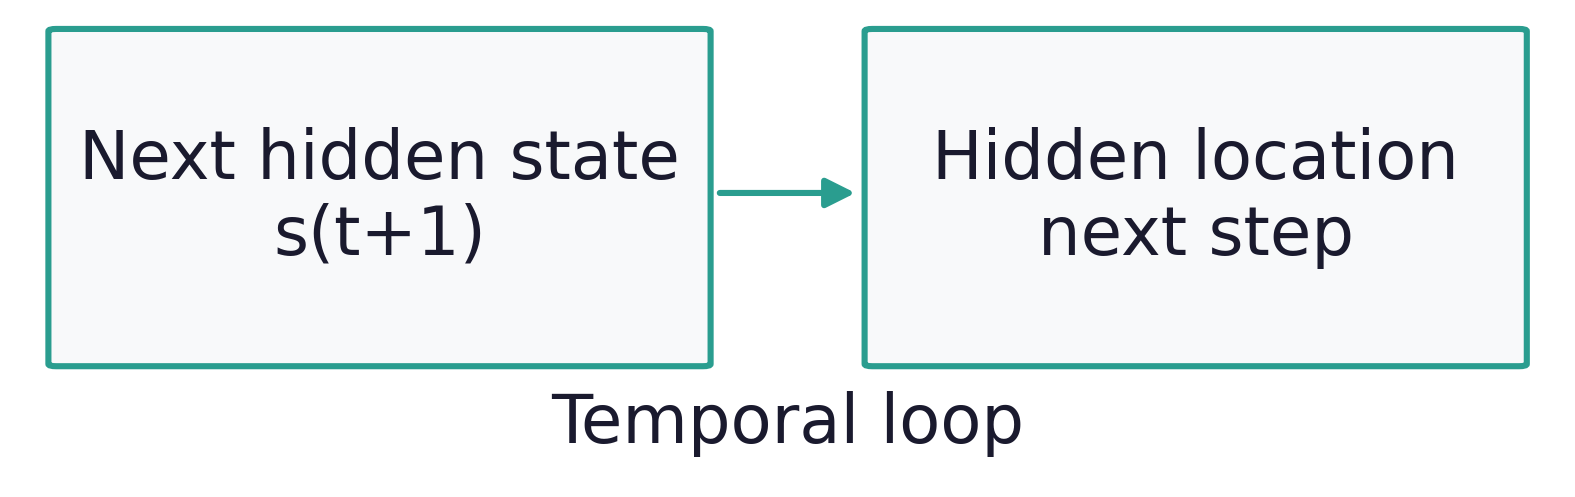
\includegraphics[keepaspectratio,width=0.98\linewidth,height=0.8\textheight,alt={Next hidden state s(t+1) → Hidden location next step: Temporal loop; data\_dependency.}]{../figures/pomdp_loop.slide-next-step.png}
\refstepcounter{figure}\label{fig:pomdp-loop-slide-panel-17}
\end{figure}
\end{frame}

\begin{frame}{Hidden-state to action loop (part 22)}
\begin{figure}
\centering
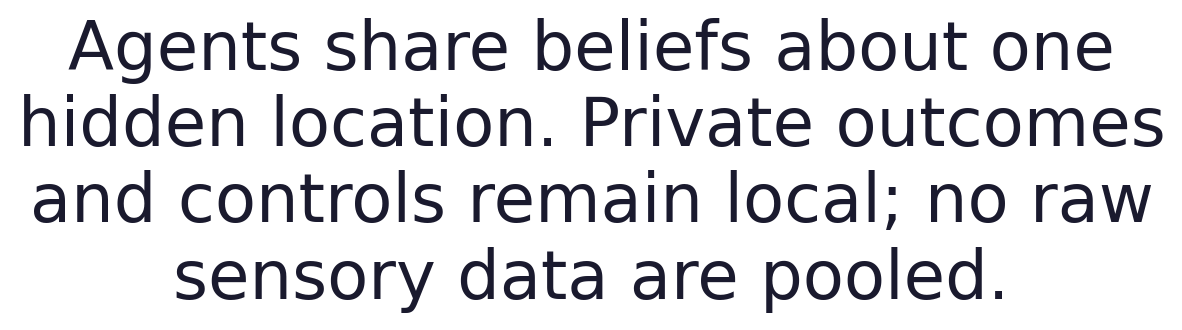
\includegraphics[keepaspectratio,width=0.98\linewidth,height=0.8\textheight,alt={Agents share beliefs about one hidden location. Private outcomes and controls remain local; no raw sensory data are pooled.}]{../figures/pomdp_loop.slide-privacy.png}
\refstepcounter{figure}\label{fig:pomdp-loop-slide-panel-18}
\end{figure}
\end{frame}

\begin{frame}{Hidden-state to action loop (part 23)}
\begin{figure}
\centering

\includegraphics[keepaspectratio,width=0.98\linewidth,height=0.8\textheight,alt={Flat federation uses inference and communication. The moving-world extension also executes B and EFE-guided control.}]{../figures/pomdp_loop.slide-optional-control.png}
\refstepcounter{figure}\label{fig:pomdp-loop-slide-panel-19}
\end{figure}
\end{frame}

\begin{frame}{Hidden-state to action loop (part 24)}
\begin{figure}
\centering
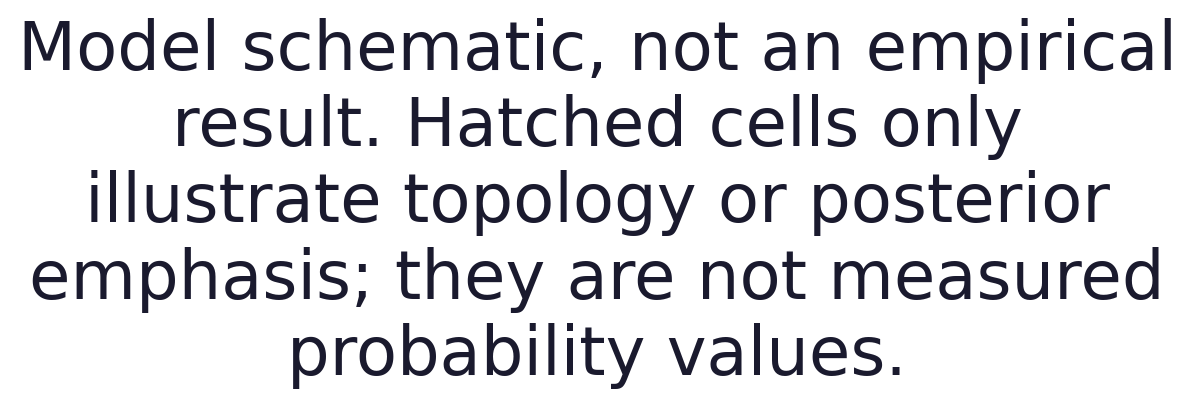
\includegraphics[keepaspectratio,width=0.98\linewidth,height=0.8\textheight,alt={Model schematic, not an empirical result. Hatched cells only illustrate topology or posterior emphasis; they are not measured probability values.}]{../figures/pomdp_loop.slide-scope.png}
\refstepcounter{figure}\label{fig:pomdp-loop-slide-panel-20}
\end{figure}
\end{frame}

\end{document}
